% XeLaTeX编译,编译参考文献引用等需两次编译。
\documentclass[openright,oneside]{ctexbook}	% 加[draft]选项可不显示图片本体,加快编译,全文完成后再删除
\makeatletter
\renewcommand\section{\@startsection{section}{2}{\z@}%
	{1.5ex \@plus1ex \@minus.2ex}%
	{.1ex \@plus.1ex}%
	{\normalfont\normalsize\bfseries}}								%% 以上4行,定义让section后自动断行
\makeatother

	\renewcommand{\chaptermark}[1]{\markboth{第 \thechapter\ 章\quad #1}{}}
	% \CTEXsetup[name={第~,~章}, nameformat={\bfseries \fangsong \zihao{4}}, titleformat={\bfseries \fangsong \zihao{4}}, number={\arabic{chapter}}]{chapter}%一级标题四号仿宋
	\ctexset { chapter = { name={第~,~章}, nameformat={\bfseries \fangsong \zihao{4}}, titleformat={\bfseries \fangsong \zihao {4}}, number={\arabic{chapter}} } } 
	
	% \CTEXsetup[beforeskip={0pt}, afterskip={20pt}]{chapter}	%章的前后行距
	\ctexset { chapter = { beforeskip={0pt}, afterskip={20pt} } }

	% \CTEXsetup[format={\heiti \zihao{-4}}]{section}	%二级标题四号黑体
	\ctexset { section = { format={\heiti \zihao {-4}} } } 

	% \CTEXsetup[beforeskip={2ex plus .5ex minus .2sex}, afterskip={0ex plus .2ex}]{section}
	\ctexset { section = { beforeskip={2ex plus .5ex minus .2sex},afterskip={0ex plus .2ex} } } 
	
	% \CTEXsetup[format={\fangsong \zihao{-4}}]{subsection}%三级标题小四号黑体
	\ctexset { subsection = { format={\fangsong \zihao {-4}} } } 

	
	% \captionwidth{0.8\textwidth}
	% \changecaptionwidth
	\CTEXoptions[contentsname={\normalfont \heiti \zihao{4}目\quad 录}, figurename={图}, tablename={表}, bibname={\zihao{-4} \normalfont \heiti 参考文献}]
	
\usepackage[titles]{tocloft}
	\renewcommand{\cftdot}{$\cdot$}
	\renewcommand{\cftdotsep}{1.5}
	\setlength{\cftbeforechapskip}{10pt}
	\renewcommand{\cftchapleader}{\cftdotfill{\cftchapdotsep}}
	\renewcommand{\cftchapdotsep}{\cftdotsep}
	\makeatletter
	\renewcommand{\numberline}[1]{%
		\settowidth\@tempdimb{#1\hspace{0.5em}}%
		\ifdim\@tempdima<\@tempdimb%
		\@tempdima=\@tempdimb%
		\fi%
		\hb@xt@\@tempdima{\@cftbsnum #1\@cftasnum\hfil}\@cftasnumb}		%% 防止目录里章节号和章节名重叠
	\makeatother

\usepackage{minted} % 使用代码高亮,必须-shell-escape



\usepackage{amsmath}	%[fleqn]可以公式不居中
\usepackage{amsfonts}
\usepackage{amssymb}
\usepackage{graphicx}
\usepackage[paper=a4paper, top=25 mm, bottom=20mm, left=25 mm, right=30mm, head=5 mm, headsep=2.5 mm, foot=5 mm]{geometry}
\usepackage{tabularx}
\usepackage{txfonts}
\usepackage{booktabs} % 三线表
\usepackage{multirow} % 多列
\usepackage{fancyhdr}    % 页眉页脚
\usepackage[numbers,sort&compress]{natbib}
	\setlength{\bibsep}{0ex}  % vertical spacing between references
\usepackage{algorithm}
\usepackage{algorithmic}
\usepackage{float}
	%1方式,线型
	\floatstyle{ruled}
	%2环境、浮动方式、包含文件(类似toc,lof,lot)
	\newfloat{algorithm}{htbp}{loa}[chapter]
	%3 目录名称,类似-->\renewcommand*{\lstlistlistingname}{程~序}
	\floatname{algorithm}{算~法} %环境名,使用方法\begin{algorithm}caption{}.......\end{algorithm}

\usepackage{caption}  % 标题
	\renewcommand\captionfont{\zihao{-5} \heiti}
	\captionsetup{labelsep=space}
	\captionsetup{justification=centering}
%	\captionsetup[figure]{options}
%	\captionsetup{labelsep=colon}
	\setlength{\abovecaptionskip}{6pt}
	\setlength{\belowcaptionskip}{-10pt}
	
% Windows	\newCJKfontfamily\fzyt{FZYaoTi}
% Mac \newCJKfontfamily\fzyt{FZYTK--GBK1-0}
	\newCJKfontfamily\fzyt{FZYTK--GBK1-0}

%后面有了	\setmainfont{Times New Roman}

\usepackage{enumitem}
	\setenumerate[1]{itemsep=0pt,partopsep=0pt,parsep=\parskip,topsep=0pt}
	\setitemize[1]{itemsep=0pt,partopsep=0pt,parsep=\parskip,topsep=0pt}
	\setdescription{itemsep=0pt,partopsep=0pt,parsep=\parskip,topsep=0pt}

		
	\pagestyle{plain}

	
	\newcommand{\dif}{\mathop{}\!\mathrm{d}} 

\usepackage{microtype}	%	microtype 宏包可以改善了单词、字母的间距。它可能做了很多,但是大部分人察觉不到使用它之后文档的变化。但至少,加载了 microtype 之后,文档看起来更好,也更容易阅读。注意:如果有使用到字体宏包,需要将 microtype 宏包放在它们的后面,因为这个宏包对单词、字母的调整和字体是有关的。

\usepackage{siunitx}	%	siunitx 宏包大大简化了写作科技文的 TeX 命令,科技文写作中很大一部分是单位、数字。这个宏包添加了一些命令,比如 \num命令可以输出我们想要的各种方式的数字形式(比如科学记数法),而 \si 命令用来输出单位。我经常用到的命令是 \SI 和 \SIrange。比如 \SI{10}{\hertz} 输出为 “10Hz”(这能有效避免输入错误,我可能会写成 HZ 或者 hz 而不是 Hz)。\SIrange 命令多一个参数:\SIrange{10}{100}{\hertz} 输出为 “10Hz to 100Hz”。


% \usepackage{hyperref}%这样可以搞出pdf书签%若不要红色边框就把这句话去掉

%默认情况下,目录链接是带红色的边框的,如果不想这样,可以:
\usepackage[bookmarks=true,colorlinks,linkcolor=black]{hyperref}



\begin{document}

	\makeatletter
	\def\@cite#1#2{\textsuperscript{[{#1\if@tempswa , #2\fi}]}}				%% 以上2行 - 把引用改上标;
	\makeatother

\begin{figure}[!htbp]
	\centering
	
\includegraphics[scale=0.11]{pic/top}
\end{figure}

\vspace{22.5pt}

\begin{center}
	{\zihao{-0} {\fzyt 操作系统课程设计}}^^^^200b \\% 这儿有个bug
	{\zihao{-0} {\fzyt 实践报告}}^^^^200b \\% 这儿有个bug

\end{center}

\vspace{42.8pt}

\begin{figure}[!htbp]
	\centering
	
\includegraphics[scale=0.4244]{pic/logo}
\end{figure}

\vspace{28pt}
\setmainfont{FZYTK--GBK1-0} % 可能不用加这句,Mac下,故没尝试
\begin{flushleft}
	\zihao{3} \fzyt 
	\renewcommand\arraystretch{1.3}
	\begin{tabular}[b]{p{1.92cm}p{2.45cm}p{3.8cm}p{1.4cm}p{3.8cm}}
		 & 题\hspace{2em}目:& \multicolumn{3}{c}{\underline{\makebox[10cm]{基于x86架构的操作系统之文件}}} \\
	   &				  & \multicolumn{3}{c}{\underline{\makebox[10cm]{系统设计与实现}}} \\
		% &				  & \multicolumn{3}{c}{\underline{\makebox[10cm]{标题不长不短刚刚好}}} \\
		% & 题\hspace{2em}目:& \multicolumn{3}{c}{\underline{\makebox[10cm]{哈哈哈哈哈哈哈哈哈座蓝桑架}}} \\
		% &				  & \multicolumn{3}{c}{\underline{\makebox[10cm]{标题不长不短刚刚好}}} \\
		& 姓\hspace{2em}名:& \multicolumn{3}{c}{\underline{\makebox[10cm]{邱\ 日\ }}} \\
		& 学\hspace{2em}院:& \multicolumn{3}{c}{\underline{\makebox[10cm]{信息科学与技术学院}}} \\
		& 专\hspace{2em}业:& \multicolumn{3}{c}{\underline{\makebox[10cm]{计算机科学与技术}}} \\
		& 班\hspace{2em}级:& \multicolumn{3}{c}{\underline{\makebox[10cm]{计\ 科 \, 151}}} \\
		& 学\hspace{2em}号:& \multicolumn{3}{c}{\underline{\makebox[10cm]{19215116}}}  \\

		% & 学\hspace{2em}号:& \multicolumn{3}{c}{\underline{\makebox[10cm]{1\,9\,2\,1\,5\,1\,1\,6}}}  \\
		& 指导教师: & \underline{\makebox[3.8cm]{姜海燕}}  & 职称: & \underline{\makebox[3.95cm]{教授}} \\
	\end{tabular}
\end{flushleft}

\vspace{\baselineskip}

\begin{center}
	\zihao{3} 	\fzyt
	\today 
	
	% 南京农业大学教务处制
\end{center}

\setmainfont{Times New Roman}
\thispagestyle{empty}	\setcounter{page}{0}
\clearpage


\vspace{2\baselineskip}

{\renewcommand\baselinestretch{1}\selectfont
\tableofcontents \par } \pagenumbering{Roman}	\addcontentsline{toc}{chapter}{目录}	\clearpage


\begin{center}
	\zihao{3} \heiti	基于x86架构的操作系统之文件系统设计与实现	\end{center}
\begin{center}
	\zihao{-4} \fangsong	计算机科学与技术专业学生 \quad 邱日\\	指导教师 \quad 姜海燕	\end{center}

\zihao{5}
\addcontentsline{toc}{chapter}{摘要}
\noindent{\heiti 摘要:}{\songti 
此次课程设计的目的在于通过在x86架构的计算机上构建简易而真实的操作系统内核,重点实现文件系统部分,来加深
对操作系统文件系统管理原理的认识,乃至对操作系统整体的理解.

在实现上,首先利用grub加载我的内核镜像,然后设置函数栈大小,段的管理上设置好gdt表,初始化idt表,采用连续内存分配.
整个内核具体涉及到处理器管理,中断和异常的处理,系统调用的实现;涉及存储管理,基于连续空间分配和回收存储空间;
涉及设备管理,编写了键盘驱动、字符显示设备的驱动、ATA硬盘驱动,内核能够操纵屏幕键盘和读写硬盘;在文件系统的实现上,
对inode索引节点采用基于位图的空间分配回收,对数据区采用基于成组链接的磁盘空间分配与回收,采用多级目录,三级索引.

通过测试用例的验证,本系统在文件系统方面实现了预期功能,"学中干,干中学",理论实践相结合,自己也提高了操作系统方面
综合能力.
} 

\addcontentsline{toc}{chapter}{关键词} 
\noindent{\heiti 关键词:}{\songti Linux; 文件系统; inode; 超级块;成组链接 } %要具体•避免罕见缩写词和一般性词汇

\vspace{135pt}

% \begin{center}
% 	\zihao{3} Design and implement of a toy-like operating system--"RiOS" \end{center}
% \begin{center}
% 	\zihao{-4} Student majoring in  computer science and technology \quad Ri Qiu\\Tutor\quad Haiyan Jiang\end{center}

% \zihao{5}
% \addcontentsline{toc}{chapter}{Abstract}
% {\renewcommand\baselinestretch{1}\selectfont
% \noindent\textbf{Abstract: }我是摘要
% 	\par}

% \vspace{-0.2\baselineskip}
% \addcontentsline{toc}{chapter}{Key words}
% \noindent\textbf{Key words: } 三; 到; 五; 个; 关键词

% \vspace{15pt}
\clearpage 

\zihao{-4} \songti	

\pagenumbering{arabic} % 阿拉伯数字页码
% \usepackage{minted}

\chapter{目的及意义} 
\pagenumbering{arabic} % 阿拉伯数字页码
构建真实的简易操作系统可以让我们更加深刻地了解操作系统是如何控制计算机的.这是本课程设计
区别于之前仿真实验的一点.本系统从内核的加载开始,完成系统中断与异常的控制,编写了键盘、屏幕
驱动;内存管理采用简单连续分配方法,实现内存分配与回收;重点实现的是文件系统,采用位示图法管理
inode,用成组链接法管理数据区,通过所编写的ATA硬盘驱动操纵硬盘,完成了目录管理和多级索引的文件管理.

本实验"小而精",简化实现细节,强调文件系统的基本原理.做完本实验能够初步形成对操作系统的
整体认识.

% \begin{minted}{c}
%     int main() {
%         printf("hello, world");
%         return 0;
%     }
% \end{minted}



% \clearpage 

\chapter{课程设计思路及完成任务} 
% \pagenumbering{arabic} % 阿拉伯数字页码
操作系统管理各种计算机硬件,为应用程序提供给基础,并充当计算机硬件与用户直接的中介,
它是硬件的第一层封装和抽象,在计算机系统中处于重要地位.
但是在实验中,大多会出现停留在应用层、不能深入到底层的情况.我认为,只有通过阅读研究
真实的操作系统源码并自己动手实践,才能较为深刻地理解原理.

\section{思路}
首先,目的明确:要造一个能够在计算机上直接运行的简易操作系统内核(不依赖于windows或Linux).
由于水平和精力所限,此次课设重点放在它的文件系统的实现上.
\subsection{开发环境}
我们操作系统内核的开发当然还是要在操作系统内进行.Linux下的工具链比Windows要完善一些,因此
选用GNU/Linux作为开发平台,笔者开发时具体选用的是Ubuntu Bionic Beaver (development branch)18.04.
是X86\_64架构.在进行本实验之前请先确保交叉编译的环境已经被正确建立起来了.

实验涉及到的开发工具有用于编译内核的gcc、x86机器的硬件模拟软件qemu,内核面向的CPU架构为IA-32,
由于x86系列芯片的后向兼容性,编译好内核还是可以在我们真实的计算机上运行,这是可验证的.
\subsection{主要特点}
\begin{itemize}
\item 编程用C和C++及少部分汇编语言
\item 面向x86,32位架构
\item 用GRUB2引导内核
\item 类似UNIX的风格
\item 文件系统面向IDE(ATA)硬盘,可读写、多级索引
\item 有简单的shell解释命令并运行
\end{itemize}
\subsection{运行流程}
\subparagraph{启动}
首先,加载内核工作从符合GRUB2的Multiboot规范的multiboot.asm开始,BIOS会对它进行进行检查,在boot.asm中,关中断
,然后跳向C语言写成的kmain.cc中的RiOS\underline{ }main函数.本系统并不是一个普通的应用层软件,
我们还需要一个链接脚本(linker.ld)来定义编译后可执行内核的结构,它定义了内核加载到
内存的位置,由于内存中前1MB含VGA显存空间、16位设备扩展ROM等预留空间,这里内核从1M
空间开始,(GRUB2的引导工作在此对程序员透明).这里有个很重要的工作就是定义C语言的调用函数时的栈大小,
不能定得过小,否则以后有可能出现栈溢出的情况,而且如果事先不知道的话将很难定位内核崩溃的原因.

\section{完成任务} 
\subparagraph{运行}
跳转到C语言写成的RiOS\_main函数以后,(当然,函数用什么写成对于编译好的二进制内核来说已经没什么意义了)
首先通过写显存的方法在屏幕打印字符,然后依次进行以下工作:
\begin{enumerate}
\item 初始化全局描述符表(global descriptor table).
\item 初始化字符设备驱动.
\item 初始化中断描述符表(interrupt descriptor table),这里设置了各个中断门,将编写好的
中断处理程序与中断向量表对应好,这里包括了键盘中断服务程序,完成了键盘扫描码的处理就可以用键盘输入了.
\item 完成定时器(8253或其兼容芯片)的设置
\item 内存管理上,通过简单连续分配实现内存的分配与回收
\item 控制台终端简易shell的实现,解释执行键盘输入的命令
\item 用类似处理中断的方法处理系统异常
\item 检测PC有多少磁盘,它假设磁盘0是存在的,因为内核就是从磁盘0加载的,然后检查磁盘1是否存在,
若磁盘1存在,就会通过写I/O端口0x1f6来选择磁盘1,本系统为了实现得更加清晰,默认磁盘0只用来存放内核并
完成加载内核的工作,内核的文件系统将建立在磁盘1上,因此请确保磁盘1存在.
\item 完成系统调用的设置
\item 初始化硬盘分区表,其中一步是检查磁盘某特定位置有无文件系统特定的Magic number,若无,则认为
文件系统尚未建立,将会格式化全盘,然后建立起整个文件系统;若Magic number存在,则不格式化,直接从
硬盘加载上次开机已写入的文件内容.
\item 于IDE(ATA)硬盘上建立文件系统,完成超级块的初始化设置,设置内存专用块,为用于数据区分配回收的
成组链接法做好准备;inode的分配回收则用位示图法;对文件采用多级索引;支持多级目录.
\end{enumerate}


% % \clearpage
 

\chapter{操作系统整体设计} 
% \pagenumbering{arabic} % 阿拉伯数字页码
我将这个简易的操作系统内核命名为RiOS.从结构上看,它实现了系统引导、字符设备驱动、
中断和异常处理、基于连续内存分配的内存管理等,重点实现了文件系统,文件系统部分是
比较完善的.由于水平及时间精力的限制,并没有实现内存分页管理,因而没有缺页调度.
不过它是可扩展的,在此基础上,如果同学们有兴趣,可以尝试分页内存管理并为它加上对多进程
的支持.

\section{操作系统内核引导}
万事开头难,如何正确引导我们的内核,在裸机上打印一行"Hello,world!"是一个简单而又复杂的事.
简单,是因为相对于复杂的内核编写工作它是最简单的;复杂,是因为第一步的跨出需要了解相关背景知识、
面临一些重要的选择,否则将无从下手.

如何加载内核?想象一下上一次装系统的情形,你应该是先将Windows镜像通过软件烧写到U盘中,然后
调整BIOS引导顺序,将U盘启动优先级调到最高,将烧写好的U盘插入电脑,重启,电脑将进入U盘中的Windows
系统.

我们要做的就是得到操作系统内核镜像,用合适版本的gcc编译好自己编写的RiOS内核代码,可以得到内核镜像,
以下工作就和上面一样了.如果你用过"老毛桃"、"大白菜"等软件装过系统,想必对模拟启动功能不陌生.
模拟启动,可以验证是否正确写入,是否能够正常启动,免得我们不断重启白忙一场.编写内核代码不可能一次成功
,我们需要类似模拟启动的功能,QEMU软件就是这样一款广泛使用的虚拟机软件,类似的还有bochs软件,他们性质
类似于Virtualbox或VMware,不过更利于我们调试内核,QEMU广泛应用于国内外的操作系统教学中.

关于引导,我们可以选择是自己写bootloader;也可以像Ubuntu那样使用成熟的GRUB来引导内核.前者我在
之前的实验中查阅相关资料作了初步探索,的确可以引导我们的小内核,但有几个缺点:
\begin{itemize}
    \item 由于x86历史复杂,我们需要背负历史包袱,在代码中要向键盘控制器8042发送命令,打开A20控制器,
这样才能避免地址的回绕,访问到1MB以外的地址.
    \item 因为默认进入的是x86的实模式,(这也是我们在熊老师的汇编语言课上一直使用的模式),我们要进入
保护模式还得费点劲,要清空指令流水线,之后要正确设置GDT表,通过长跳转才能正确进入32位保护模式.
    \item 需要调用BIOS的中断服务程序来将代码从外存拷贝到内存,拷贝过程涉及磁盘的柱面、磁头、扇区,还
需要知道自己U盘的这些参数具体是多少.理论上可以通过查询的方法得到,但之前我为了简单先通过软碟通软件得知这些
参数然后硬编码,这样不利于通用性.
    \item 通过BIOS的中断服务程序调用来拷贝内核,这种方法支持的最大拷贝容量很小,哪怕之后由通过柱面号、
磁头号、扇区号访问的方式改为磁盘LBA访问方式,拷贝容量仍然不是很大.随着代码增长和内核增大,有可能出现
拷贝不完全的现象,内核不能全部加载到内存,将出错.
    \item 以上实现虽然可能只需要一百多行汇编代码,但需要了解相关背景知识,只要有一点写错,就不能成功
引导,代码很难调,关键是我觉得这些与操作系统原理本身关系不是很大,主要是由x86的悠久历史和向后兼容引起的麻烦
,我们没有必要在这上面花费过多时间.    
\end{itemize}
因此在本次课程设计,我选用了GRUB2引导我们的内核,GRUB2也是Ubuntu系统默认的引导方式.这样我们可以专心
内核的编写了.
\subsection{BIOS中断服务程序}
操作系统的引导是从BIOS开始,计算机加电后,BIOS在执行了一系列硬件检测和初始化操作后会将ROM中的64KB代码复制到
内存低端的1M末端的64K处,然后跳转到此地,并让CPU进入实地址模式工作,然后BIOS将会从硬盘或其他块设备将操作系统
引导程序加载到内存0x7c00处,并跳转到这里继续执行引导程序.BIOS会判断我们插入的U盘MBR主引导扇区偏移511处是否为
0x55及偏移512处是否为0xaa,若不满足则认为不可引导,否则将会把它加载到内存0x7c00处.若我们自己编写bootloader,则我们需要确保引导扇区的
代码不超过512字节,我们的整个内核当然会超过512字节,因此需要在这512字节的代码中完成把内核代码全部从外存调入内存的工作.
这里可以使用BIOS中断服务程序,具体可以是BIOS int 13h调用,它是BIOS提供的磁盘基本输入输出中断调用,它可以完成
磁盘读写、校验、格式化等,它历史悠久,采用的是CHS寻址方式,因此最大只能访问8GB左右的硬盘.本课程设计不使用这种方法.
\subsection{GRUB2}
GRUB是GNU GRand Unified Bootloader的缩写,是GNU计划的一个成熟的引导程序包,用它可以实现多操作系统的引导.
这里我们使用GRUB2,只要我们符合多引导头(multiboot header)的规范,它就能将我们带入32位保护模式.
\paragraph{Grub安装到U盘方法}
首先在Ubuntu系统安装grub2,然后插U盘,通过Linux命令安装grub2到U盘
\begin{minted}{shell}
# 首先插入U盘
df -h # U盘是/dev/sdb
sudo mount /dev/sdb /mnt #挂载U盘到/mnt
mkdir /mnt/boot 
sudo grub-install --root-directory=/mnt /dev/sdb
#出现提示错误信息 grub-install: error: will not proceed with blocklists.
#不管他,强制 块列表是不可信赖的,不推荐使用。问题依旧,输入一下指令,强制写入。
sudo grub-install --force --root-directory=/mnt /dev/sdb
\end{minted}
如图~\ref{grub}~所示。

\begin{figure}[!htbp]
	\centering	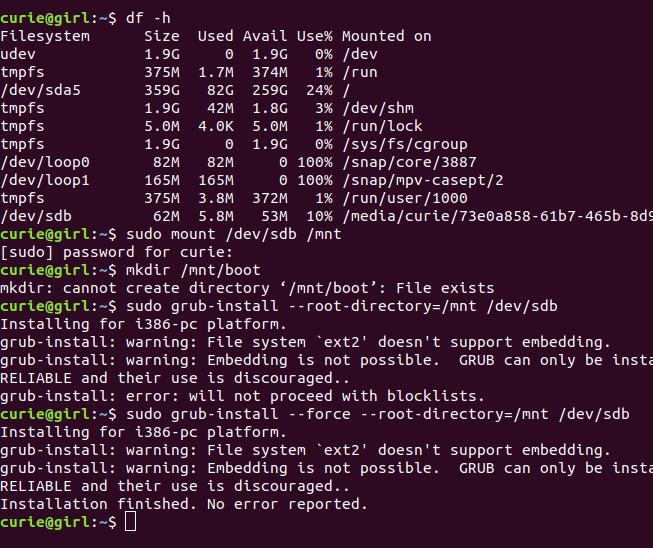
\includegraphics[width=12cm]{pic/assets/grub}
    \caption{grub2安装到U盘过程}	\label{grub}	\end{figure}
Grub的配置文件grub.cfg应当按照相关规范编写,并不困难.
\subsection{Multiboot规范}
Grub引导程序将会检测我们内核是否符合Multiboot头的规范,这里应当查阅相关GNU官方手册,
我们采用较新的Grub2,用到的域有'magic','architecture','header length','checksum'
等几项,对于Grub2,魔法数字(magic)域是32位的0xe85250d6;架构(architecture)域上,我们是
i386保护模式,是0(32位),若是MIPS架构,则这项为4;32位的'checksum'域主要起检查作用,应当保证
'checksum'域和以上的三个域加起来为0,这样Grub才认为Multiboot头正确地写好了.这之后依次还有16位
的'type'域、16位的'flag'域、32位的'size'域,我们令它们分别为0,0,8即可.

\subsection{链接脚本}
我们需要精确控制内核各部分日后加载在内存的位置,因此用来描述输入文件中的各个段(数据段、代码段、堆、栈、bss)
如何映射到输出文件的链接脚本必不可少.链接器是要使用链接脚本的,若不手动提供,它会使用默认的链接脚本.
通过汇编器及gcc编译完我们的诸多代码文件,会得到很多目标文件,通过链接脚本定义的方法,我们将它们有效地组织起来,
最终输出单个的内核镜像.在脚本中,通过OUTPUT\_FORMAT指明输出格式,ENTRY指出入口为boot.asm中
的标号RiOS\_start所在位置.由于CPU低地址有许多预留给系统,故应该把前1MB内存腾出来,内核从1MB后
开始.这部分背景知识可阅读《Linux内核完全注释》.
IBM PC兼容机内存使用如图~\ref{memory}~所示。
\begin{figure}[!htbp]
	\centering	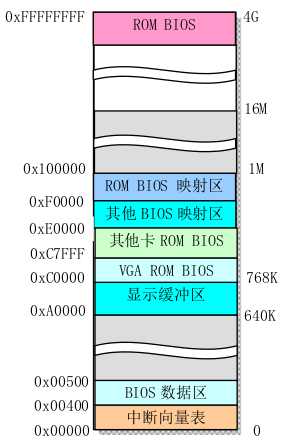
\includegraphics[width=6cm]{pic/assets/memory}
    \caption{内存使用情况}	\label{memory}	\end{figure}

.text区是代码段;.data区是数据段;.bss段则存放那些还没有被初始化的全局变量,BSS是
'Block Started by Symbol Segment'的缩写.

\subsection{Makefile文件}
Makefile是make工具使用时的配置文件,make工具能够自动决定一个含有很多源程序文件的大型程序中哪些文件需要重新编译.
Makefile的使用较为复杂,这里简要介绍一下背景以及本工程的Makefile的编写,关于Makefile的更多写法请阅读GNU make
使用手册.

从Makefile中可以大致看出RiOS的整个框架结构.内核主要由C或C++及汇编构成.在汇编语言课程学习中,我们使用了DOS环境
下MASM汇编器,不过它并不适合我们在Linux环境下交叉编译内核汇编代码.还有很多其他的汇编器,在Linus最初版本的Linux中
,他使用了两种汇编器as86和gas,as86专为Minix和Linux设计,现在应该算过时了,gas是GNU计划的自由软件,作为gcc的一个
后台设计.

本Makefile中使用了grub-mkrescue命令,请确保系统中xorriso已经安装(sudo apt-get install xorriso).

\subsection{汇编器}
我们的RiOS也使用了两种汇编器:NASM和gas.NASM是一个为可移植性和模块化而设计的一个80x86汇编器,
它支持相当多的目标文件格式(包括ELF、a.out、Microsoft 16-bit OBJ等),和Intel语法相似但更简单.(我们在熊老师汇编课上学习的应该算Intel语法)
NASM对宏命令支持相当不错,而且错误检测功能应该优于gas,我们要生成ELF格式的文件,它更加合适.而gas和gcc联系密切,
我们可以较方便地使用内联汇编.因此C编译器采用gcc,汇编器采用NASM及gas,链接器使用ld,另外用make工具完成自动编译.

Makefile中通过.PHONY定义了一些伪目标,比如help、run、clean等,这样make和他们搭配使用,如make help等就能实现相应功能.
内核主要分为内存管理模块、核心模块、块设备模块、字符设备模块、应用层模块等.鉴于之前有编译中间目标文件(.o)过多,和源代码混在一起
,不方便管理的缺点,这次仔细设计内核编译的结构,cd到代码顶层目录第一次敲make时将另外建立build文件夹,将在里面递归建立文件夹,存放中间编译
文件的build文件夹结构组织将和存放代码的src文件夹结构相同,这里使用了Makefile的自动变量功能.这样代码与中间文件分开,结构也比较清晰.

\section{汇编与C的相互调用}
\subsection{从汇编到C语言}
为了减少汇编代码量,提高效率,我们应当尽快过渡到C语言.C语言的函数调用基于栈,只有设置号合适的
函数栈大小和地址,才能有效地实现C语言的函数调用.在之前的计算机图形学课程中的种子填充算法中,我们体验过
栈溢出导致的程序崩溃,所以考虑到有些函数将使用较多的栈空间,我们不应吝惜开始预留的栈空间.内核编写中,
有过这样的体验:当函数调用空间消耗较大时,莫名其妙内核崩溃了,但从代码上找不出任何逻辑错误.栈预留16KB可能
差不多了,但为了避免"stackoverflow"的悲剧,我预留了16MB.关中断,然后将esp指向要设置的栈顶位置,再通过
call调用C语言里编写的RiOS\_main函数去.这里的call应是一去不复返了.这样就完成了汇编到C语言的切换.
通过汇编mov指令或者是通过C语言的指针写显存,我们都可以在屏幕打印字符,将内核复制到装有grub的U盘指定位置,
插入U盘,调整启动顺序,计算机重启可以进入U盘中的内核,实现裸机的Hello,World.
Hello,World 如图~\ref{hello}~所示。
\begin{figure}[!htbp]
	\centering	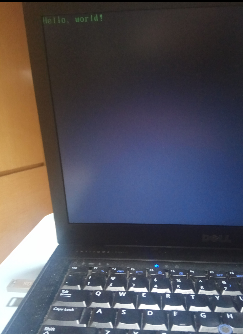
\includegraphics[width=6cm]{pic/assets/hello}
    \caption{裸机上的Hello,World!}	\label{hello}	\end{figure}
\subsection{从C到C++}
我们已经从汇编进入C语言,但是我们如何使用C++语言呢?在之前的实验中,我的探索失败了,当时我发现汇编调用不了C++
的代码,把C++代码反汇编过来会发现,与C语言不一样的是:若C语言中写一个名为foo的函数,反汇编过来是foo的标号,
而在C++中这样做则会在foo这个标号加上前缀后缀.因此若在汇编代码中调用foo函数,用foo标号按图索骥在C语言行得通,
而C++由于标号变了,就会出现'undefined'的错误.

要解决这个问题不难,但我知识浅薄,之后才发现,我应当使用在函数声明中使用extern "C".这样C++才可以调用其他C
语言代码.加上extern "C"后,会指示编译器将这部分代码按C语言的进行编译,而不是C++的.请注意是函数的声明,
不是函数的定义,因此 extern "C"主要放在头文件内.这样一来,就可以方便地使用类了.然而对于开发简易内核的我们,
使用C++可能并不是一个很好的选择.不要高兴太早,真正完全的C++的支持需要操作系统帮忙,比如异常是用不了的,它要求
运行时的支持以及内存管理的支持.类的构造和析构应该也需要内存管理的支持,然而刚刚引导时,我们尚未写相关代码,这是
个先有鸡还是先有蛋的问题.C语言更适合底层,Linux内核编写也选择的是C语言而不是C++,在此我只是探索,实际也还是
C语言风格,并未用到很多C++特性.
\paragraph{*.CC文件} 你可能注意到代码中大部分是.cc后缀的代码文件,这和我们熟知的.cpp文件其实是一样的.cc文件是Linux/UNIX下
为C++源文件默认的扩展名,不过请还是不要将它改为cpp文件,否则gcc可能不能正确识别.
\paragraph{汇编语言} 虽然在汇编语言课程中已经学过汇编语言,然而光了解8086汇编是远远不够的,386以后体系结构有所
变化,要编写面向x86(i386以后)的内核,应当了解这部分背景知识,包括之后在8086基础上新增的段寄存器等.

\section{段描述符}
bootloader接手BIOS后,开始PC系统处于16位的实模式,若自己写bootloader,还有一个切换的过程,而现在GRUB将直接把内核带
入32位保护模式.只要在32位保护模式下,才能突破实模式可使用物理内存空间不超过1MB的限制,最多可管理4GB内存;才能使用分段存储
管理机制.分段机制涉及这几方面内容:逻辑地址、段描述符(描述段的属性)、段描述符表、段选择子.

段选择子涉及段寄存器,用于定位段描述符表中表项的索引.段描述符表是段描述符的一个数组,段描述符表的长度可变,最多可包含8192个8字节描述符.有两种描述符表
:全局描述符表GDT和局部描述符表IDT.
\subsection{全局描述符表GDT (Global Descriptor Table)}

GDT本身只是线性地址空间中的一个数据结构,GDT的基线性地址和长度值必须加载进GDTR寄存器中.
GDT的基地址应当是内存8字节对齐的.《从实模式到保护模式》一书中给出了存储器的
段描述符格式:见图~\ref{gdt}~.

\begin{figure}[!htbp]
	\centering	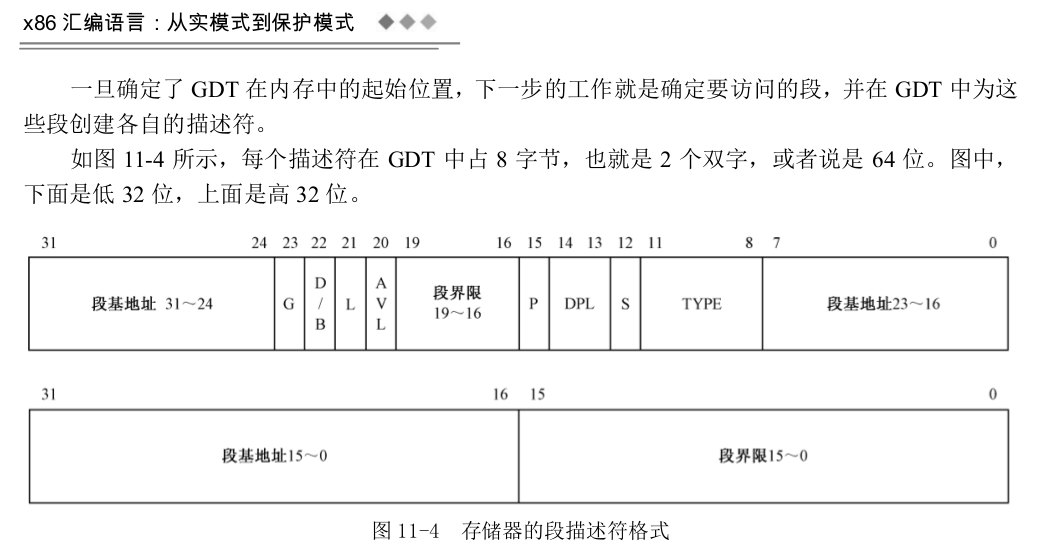
\includegraphics[width=14cm]{pic/assets/gdt}
    \caption{段描述符格式}	\label{gdt}	\end{figure}

段描述符这个格式比较复杂,一部分原因是x86历史较长,为了后向兼容,有时一个简单的
数据项往往要拆成几处,这样看起来就比较乱了,不过写代码时要严格按照硬件上的结构来,
不能出现哪怕一位的差错.



再来一个类似的段描述符结构的图:如图~\ref{segment_descriptor}~所示

\begin{figure}[!htbp]
	\centering	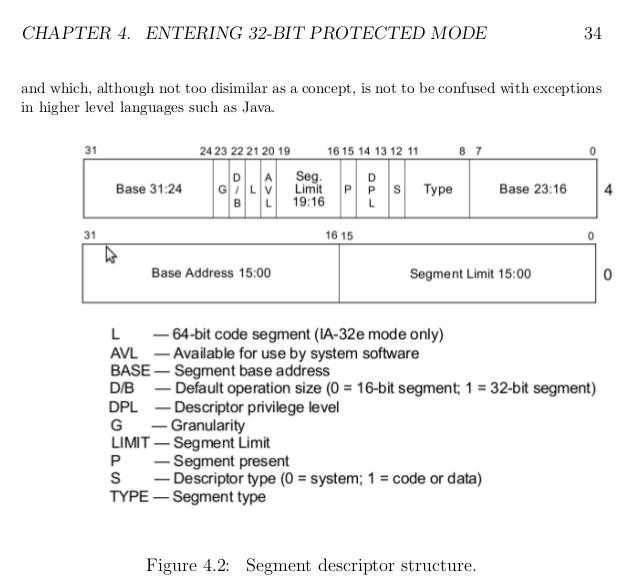
\includegraphics[width=14cm]{pic/assets/segment_descriptor}
    \caption{段描述符的结构}	\label{segment_descriptor}	\end{figure}


GDT表中的一项是64位(8B);而GDTR寄存器用来存放全局描述符表32位线性地址和
16位表长度值,故GDTR长度是48位.关于GDT及GDTR的介绍可见维基百科Global\underline{ }Descriptor
\_Table词条,亦可见《LInux内核完全剖析》76页介绍,图~\ref{wiki_gdt}~为48位的GDTR的结构.
\begin{figure}[!htbp]
	\centering	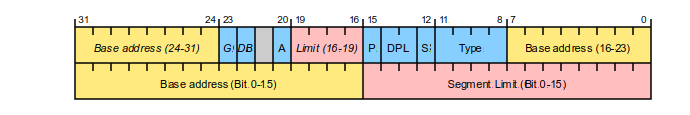
\includegraphics[width=14cm]{pic/assets/wiki_gdt}
    \caption{GDTR寄存器的结构}	\label{wiki_gdt}	\end{figure}
   
对应以上结构,RiOS中GDT表项的结构如下:
\begin{minted}{c}
struct GDT_entry 
{
u16 limit1;      /*0-15*/		
u16 base1;       /*16-31*/
u8 base2;        /*32-39*/
u8 access;       /*40-47*/
u8 granularity;  /*48-55*/
u8 base3;        /*56-63*/
} __attribute__((packed));  
\end{minted}    
GDT表项是64位,但是GDTR寄存器是48位,我们需要lgdt(Load GDT Register)
指令加载全局描述符表寄存器GDTR,把GDT表的基地址和长度从内存加载到GDTR中.
RiOS中GDT\_pointer结构由基地址和长度组成.将在RiOS/src/kernel/gas/gdt.S
中的update\_gdt函数用一条汇编指令lgdt (gdt\_pointer)完成加载到GDTR的工作.
\begin{minted}{c}
struct GDT_pointer
{
u16 limit;
u32 base;
} __attribute__((packed));
\end{minted}  

举一个段间长跳转的例子,例如用AT\&T语法写(gas)是
\mintinline{gas}!ljmp $section, $offset!

,而intel语法为
\mintinline{asm}!jmp section:offset!
.具体如
\mintinline{nasm}!ljmp $0x8, $protcseg!
,ljmp的格式是: ljmp 段选择子,段内偏移.上句指令的意思是:用0x8作为段选择符,
到gdt中去取出gdt[0x8]的值,再加上偏移量protcseg. 跳转到gdt[0x8] + \$protcseg
的地址处执行。 
\subsection{局部描述符表LDT (Local Descriptor Table)}
发生任务切换时,LDT会更换成新任务的LDT,但GDT不会改变.由于时间精力有限,本项目目前并未涉及,但
日后若要加入对多任务和虚拟内存的支持,应当研究好这一块.
\section{中断描述符表IDT (Interrupt Descriptor Table)}
在保护模式下,中断门描述符表(IDT)中断每个表项由8个字节组成,其中每个表项叫做一个门描述符
(Gate Descriptor).在IDT中,可以包含如下几种类型的系统段描述符:
\begin{itemize}
    \item 中断门描述符(Interrupt-gate descriptor)
    \item 陷阱门描述符(Trap-gate descriptor)
    \item 任务门描述符(Task-gate descriptor)和调用门描述符(Call-gate descriptor)
\end{itemize}
其中中断门描述符和陷阱门描述符的类型码分别为110和111.

\subsection{门描述符}
以下为RiOS中门描述符的数据结构,以上几种门描述符都可以是这种类型.这里使用\mintinline{gas}!
#pragma pack(1)!设置结构体的边界对齐为1个字节,也就是所有数据在内存中是连续存储的,因为这和硬件直接相关,需要精确控制到"位".
\begin{minted}{c}
#pragma pack(1)
struct GATE_DESCRPTOR{
u16 offset_lowerbits        :16;// offset bits 0..15
u16 selector                :16;// a code segment selector in GDT or LDT
u8  zero                    :8 ;// unused,set to 0
// type and attributes, total u8 type_attr;
u8  seg_type                :4 ;
u8  storage                 :1; // set to 0 for interrupt and trap gates 
u8  descr_privilege_level   :2;
u8  present                 :1;
u16 offset_higherbits       :16;// offset bits 16..31	
};
#pragma pack()
\end{minted}

中断描述符表的前32项应当留给处理器内部的异常处理.80386把中断号0至31分配
给陷阱、故障和不可屏蔽中断,把32至47之间的中断号分配给可屏蔽中断。
可屏蔽中断的中断号是通过对中断控制器的编程来设置的。

\begin{tabular}{|c|c|c|}% 通过添加 | 来表示是否需要绘制竖线
    \toprule
    Exception \# & Description & Error Code?\tabularnewline
    \midrule
    0 & Division By Zero Exception & No\tabularnewline
    1 & Debug Exception & No\tabularnewline
    2 & Non Maskable Interrupt Exception & No\tabularnewline
    3 & Breakpoint Exception & No\tabularnewline
    4 & Into Detected Overflow Exception & No\tabularnewline
    5 & Out of Bounds Exception & No\tabularnewline
    6 & Invalid Opcode Exception & No\tabularnewline
    7 & No Coprocessor Exception & No\tabularnewline
    8 & Double Fault Exception & Yes\tabularnewline
    9 & Coprocessor Segment Overrun Exception & No\tabularnewline
    10 & Bad TSS Exception & Yes\tabularnewline
    11 & Segment Not Present Exception & Yes\tabularnewline
    12 & Stack Fault Exception & Yes\tabularnewline
    13 & General Protection Fault Exception & Yes\tabularnewline
    14 & Page Fault Exception & Yes\tabularnewline
    15 & Unknown Interrupt Exception & No\tabularnewline
    16 & Coprocessor Fault Exception & No\tabularnewline
    17 & Alignment Check Exception (486+) & No\tabularnewline
    18 & Machine Check Exception (Pentium/586+) & No\tabularnewline
    19 to 31 & Reserved Exceptions &\tabularnewline
    \bottomrule
\end{tabular}

以上为0到31号分配给陷阱、故障和不可屏蔽中断的具体情况,这部分编写和中断类似,
举一个除0异常的例子,代码中出现除以0的情况,将会陷入系统异常的处理例程,系统发生panic,
打印出错信息,内核停机(halt).

如图~\ref{divisionbyzero}~.

\begin{figure}[!htbp]
	\centering	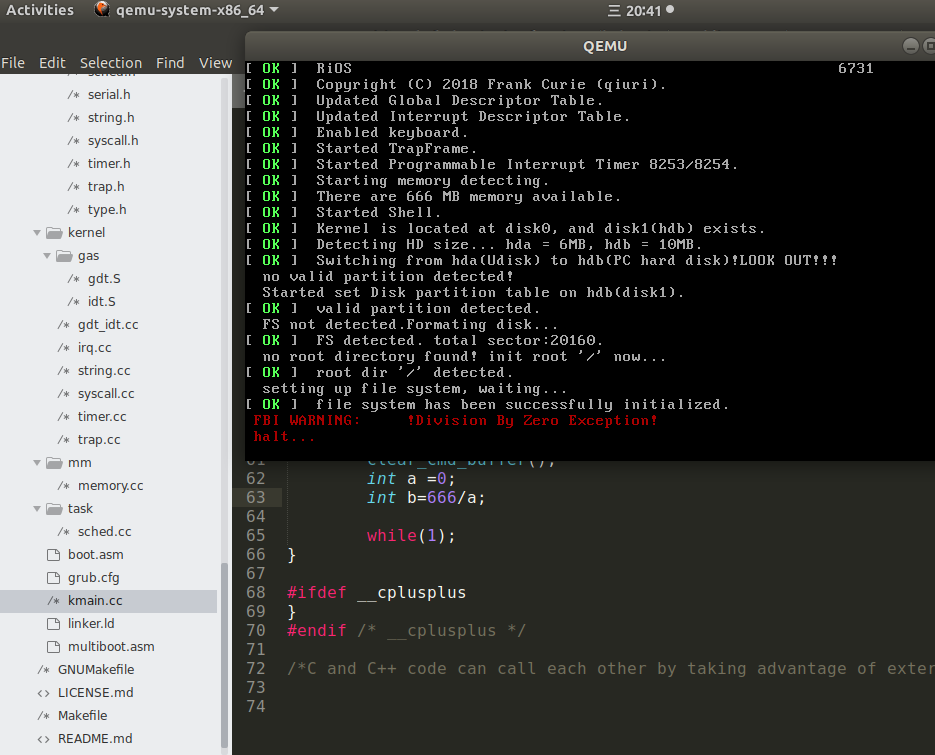
\includegraphics[width=14cm]{pic/assets/divisionbyzero}
    \caption{除0异常}	\label{divisionbyzero}	\end{figure}

IDT表中的项类似于GDT表中的项,它们都是64位长,都有基地址,都有访问标志位;然而IDT没有类似
GDT中的段限长(limit).

如图~\ref{interrupt_trap_gate}~.

\begin{figure}[!htbp]
	\centering	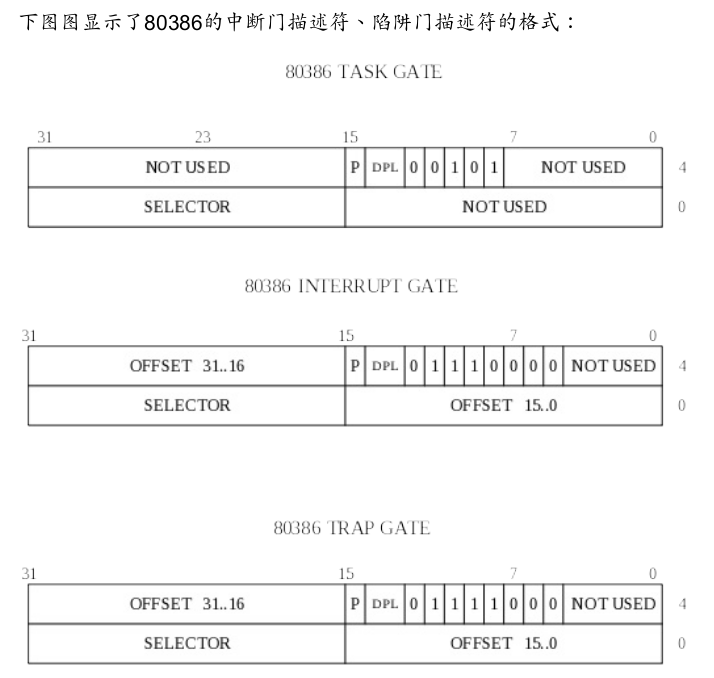
\includegraphics[width=14cm]{pic/assets/interrupt_trap_gate}
    \caption{门描述符1}	\label{interrupt_trap_gate}	\end{figure}

其他资料上类似的还有图~\ref{IDT_Gate_descriptors}~.
\begin{figure}[!htbp]
        \centering	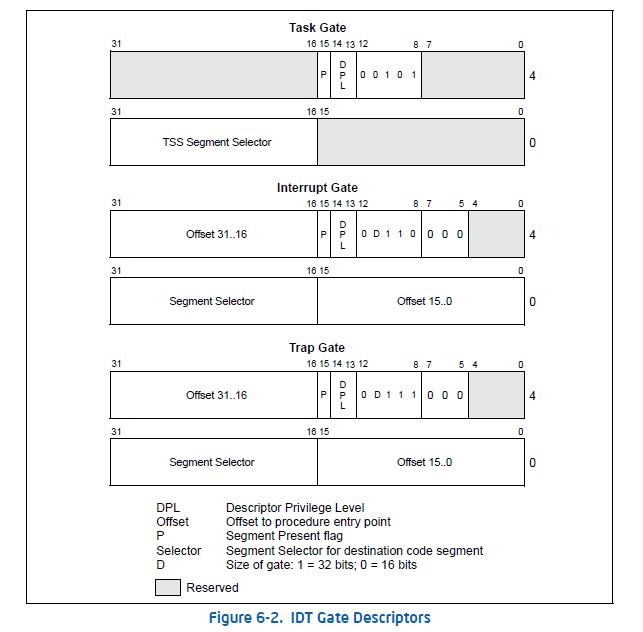
\includegraphics[width=14cm]{pic/assets/IDT_Gate_descriptors}
        \caption{门描述符2}	\label{IDT_Gate_descriptors}	\end{figure}

我们的IDT表设置了256项,当触发中断的条件满足,将会利用中断向量号查IDT表,然后转入相应
的中断服务程序,处理完再返回.如果考虑不严密,将会出现这样的情况:尚未写某个中断的处理程序,
然而相应中断或异常发生,查IDT表不知道转入到什么地方执行了,系统会因此崩溃,具体体现就是
只要这个中断触发,就会无限循环地重启.为避免这种情况发生,我们可以先把所有256项都填满,
先占个坑位;对于尚未编写的中断,统一转到一个什么也不干的中断服务程序(汇编语言编写的idt.S中的
asm\_all\_trap函数).每当我们实现一个新的服务函数,才做出相应修改,转到新写的函数中.
这部分需要把汇编语言编写的idt.S、gdt.S及用宏定义包装汇编以便于C语言调用的头文件x86.h结合起来看.
这里使用了一些汇编语言和C语言或C++相互调用的小技巧,另外需要理解栈帧的相关概念.



\paragraph{键盘中断服务程序}

\section{栈帧}
数据结构课程中的栈在硬件也有体现,x86CPU架构有专门的'push'、'pop'指令来完成入栈出栈的
操作.在x86中栈是向下增长的满栈(full descending stack),C语言的函数调用离不开
栈,GCC编译器规定的函数栈帧(stack frame)是一块存放某函数的局部变量、参数、返回地址
和其他临时变量的内存空间,图~\ref{stackframe}~为栈帧的大致结构.
\begin{figure}[!htbp]
    \centering	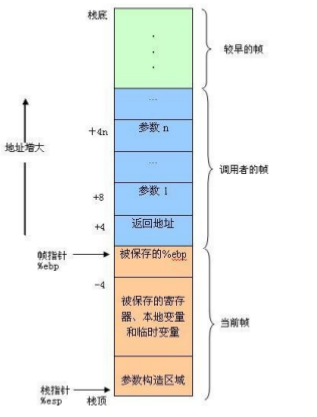
\includegraphics[width=6cm]{pic/assets/stackframe}
    \caption{栈帧结构}	\label{stackframe}	\end{figure}

\subsection{内核栈上的陷阱帧(TrapFrame)}
RiOS中的陷阱帧结构如下:
\begin{minted}{c}
struct TrapFrame{
/*registers that pushed by "pushal",xxxesp is useless */	
  u32 edi,esi,ebp,xxxesp,ebx,edx,ecx,eax;
/*below are defined by x86 hardware:eip cs .. eflags*/
  u32 err;/*irq*/
  u32 eip; 
  u16 cs; u16 padding;
  u32 eflags;
};
\end{minted}
为什么会这样?这里要先分析一下中断处理过程:

中断发生以后,CPU在通过查询IDT表跳转到中断处理例程之前,将在内核栈中依次压入错误码
(可选)、eip、CS和EFLAGS,这对应RiOS中TrapFrame结构的err、eip、cs和padding(因为字节对齐)、
eflags,其中err对应的错误码是我们手动压入的,通过不一样的错误码,可以判别到底发生何种错误.
而后面3个为x86硬件决定,顺序也是定死了的.中断后内核栈发生了变化,可以看到RiOS里一些函数以
TrapFrame结构体为传入参数,例如
\mintinline{asm}!void irq_handle(TrapFrame *trapframe);!
C语言函数传参就是通过栈实现的.这样他们可以从内核栈中把压入栈的TrapFrame"掏"出来使用.
中断发生时,将通过查IDT表跳转到各个中断对应的中断处理程序,就是在汇编写成的RiOS/src/kernel
/gas/idt.S定义的一堆名字中带handler的程序,这些handler各自压入独特错误码,然后统一转入asm\_
all\_trap函数.这仿佛一个陷阱,把所有handler都栽进去了,asm\_all\_trap到底做了什么?
\begin{minted}{gas}
asm_all_trap:
    pushal 
    push %esp
    call irq_handle
    pop %esp
    popal
    add $4,%esp
    iret
\end{minted}
可见它先pushal,先把很多寄存器的值压入栈,注意这对应TrapFrame结构的edi、esi、ebp、xxxesp、ebx、edx、ecx、eax
.另外此处的xxxesp并没有什么用.中断过程我们要密切关注栈里到底压入了什么.asm\_all\_trap这样写的目的就在于
,通过给栈中压寄存器们的值,使内核栈看起来就好像压入了一个陷阱帧结构,这样那些函数才能够从栈中
"掏出"陷阱帧.call irq\_handle函数以后,转入RiOS/src/kernel/trap.cc中的C语言函数,此函数
判断栈中的(或者说传入的参数)陷阱帧的标志码(err)是多少,然后转入相应的中断处理函数.

由于时间精力的限制,我没有写进程切换,不过基础设施已经大致搭好.日后同学们若要实现多进程,应当把中断处理过程分析清楚.
在trap.cc中的irq\_handle函数中timer\_8253\_handler\_main函数是时钟中断的处理函数,它包着do\_timer函数,进程调度
就应该改写do\_timer函数,在里面进行进程切换.

call irq\_handle以后转入irq\_handle根据err值执行不同中断服务程序,运行完还回到asm\_all\_trap,做中断最后
的恢复现场工作,既然之前
\mintinline{gas}!pushal push %esp!
,那么现在就要
\mintinline{gas}!pop %esp popal!
.为何要add \$4呢?别忘了,之前idt.S里那些一群handler们可是先压入了独特的标志码(err)的,那么现在要
恢复内核栈就要加回来.如果你之前还想再多压一些信息进栈,这里就要多加.总之,这是一个对称的过程,目的是恢复内核栈.

\section{字符设备驱动}
\subsection{屏幕}
\paragraph{光标的设置} 光标跟随输入的字符而移动,这件事不是天经地义的,它的实现也需要我们写相关代码.
VGA显卡内部有一系列寄存器可以用来控制显卡的状态。在标准的PC机上,
0x3d4和0x3d5两个端口可以用来读写显卡的内部寄存器。方法是先向0x3d4端口写入要访问的寄存器编号,
再通过0x3d5端口来读写寄存器数据。存放光标位置的寄存器编号为14和15。两个寄存器合起来组成一个16位整数,
这个整数就是光标的位置。比如0表示光标在第0行第0列,81表示第1行第1列(屏幕总共80列)。 
以下代码截取的是RiOS/src/console/console.cc中set\_cursor函数的代码,用于设置光标.

\begin{minted}{c}
Vx = xyindex%80;
Vy = xyindex/80;
u16 tmp = (Vy*80)+Vx;
outb(0x3d4,0x0f);
outb(0x3d5,(u8)(tmp & 0xff));/*cursor low port:reg15*/
outb(0x3d4,0x0e);
outb(0x3d5,(u8)( (tmp >> 8) & 0xff));/*cursor high port:reg14*/
\end{minted}    
\subsection{键盘}
\section{定时器(8253芯片或其兼容芯片)的设置}

微机原理课程学完之后不知道有什么用处,当我写本项目时才觉得还是有用的.
8253芯片和8259芯片的设置在本实验中都要用到,这里用宏定义或内联汇编把
in、out指令包装起来在C语言中用,实际上还是微机原理的那一套,初始化字
的写入等可以查阅相关资料,这里不详细展开了.

8253的初始化设置如下.
\begin{minted}{c}
void init_8253()
{
	outb(PIT_COMMAND_REG,0x34);
/*bin(0x34)='0b110100'= 00   11    010   0
 *Channel 0 ,Access mode: lobyte/hibyte , Mode 2 (rate generator),16-bit binary 
 */	
	outb(PIT_CHANNEL0_DATA_PORT,0x9c);/*low byte*/
	outb(PIT_CHANNEL0_DATA_PORT,0x2e);/*high byte*/
/* 1193180/100 = 11930 ,100HZ => a irq every 10ms
 * 11930 = 0b 0010 1110 1001 1010,first write lower bits,then the higher
 * see my guide.md and https://wiki.osdev.org/Programmable_Interval_Timer
 */	
	enable_8253();
	msg_8253_ok();
}
\end{minted}    
\section{块设备驱动}
操作系统需要和周边的输入输出设备通信,"存储程序,程序控制",操作系统应当具有管理和存储
长期保存数据的软件功能,这就是文件系统.文件系统不是空中楼阁,必须先对硬件进行封装,
这就是块设备驱动程序的意义.

使用fopen、fprintf不是很简单吗?然而这是所在的操作系统给我们封装好的库函数,我们在
实现一个简易操作系统内核,所有这些库函数都是不能用的,我们需要从底层往上逐步实现他们.
离开这些库函数,我们还能怎样操纵硬盘,读取写入数据?

I/O控制方式有:轮询方式、中断方式、DMA方式、通道方式.嵌入式系统这类课程常常会谈到"串口",原因就在于"串口"相对比较简单.
x86架构下,我们还有in、out指令来操纵外设,操纵外设需要了解外设与CPU通信的协议,高级点的我们做不了,就采用简单的中断方式,
使用in out指令来完成对硬盘的读写.
图~\ref{ports}~为常见的端口地址.来自百度百科词条"寻址空间"下'端口地址分配'
\begin{figure}[!htbp]
    \centering	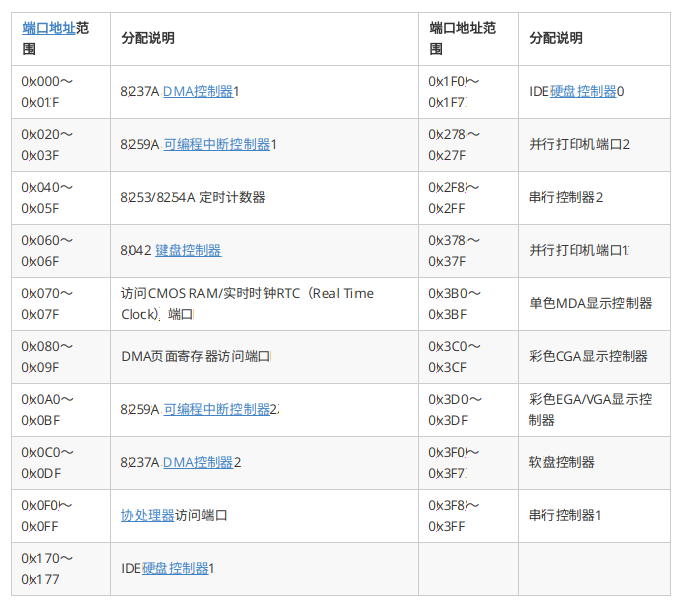
\includegraphics[width=12cm]{pic/assets/ports}
    \caption{端口地址分配}	\label{ports}	\end{figure}

其中端口0x1F0至0x1F7用于IDE硬盘控制器0,写IDE硬盘驱动主要用到它.

\subsection{IDE(ATA)硬盘}
这是一种规范,大多数情况下,IDE和ATA是同义词,IDE用得多一点,但实际上叫ATA可能更合理.
注意,这里我们讨论的是硬盘方面的IDE,并不是讨论集成开发环境的那个IDE.
以下是来自osdev网站的相关介绍(https://wiki.osdev.org/Category:ATA):

The name IDE is often used interchangeably with ATA, but "IDE" actually refers to only the 
electrical specifications of the signals on the 40 / 80 pin disk cable. ATA is the proper 
name for the entire specification.


\section{文件系统设计与实现}
下一章详细说明.


% \section{引用示例}

% \section{引用示例}
% \subsection{垃圾}
% 垃圾

% \section{引用示例}

% \clearpage 

\chapter{文件系统部分设计与实现} 
% \pagenumbering{arabic} % 阿拉伯数字页码
\section{文件系统总体设计}
我们的简单内核目前肯定支持不了其他USB设备(除引导内核用的之外),不能进入系统后从USB设备拷贝文件,所以目前我们只能有两种方式可以
新建文件,一是从键盘输入,二是从内核而来.键盘输入显然有限,输入几MB字符不太现实,故需要从内核拷贝.这样才能
达到创建较大文件,测试文件系统的目的.这要保证静态内存分配的bss段要足够大.


我们要操纵的硬盘是哪一个呢?若是真实物理机测试的话,内核是存放于U盘的,我们的文件系统或许可以和内核
合成一块,做成系统集成盘,就像赵炯《Linux内核完全注释》中Linux0.11的实验环境一样.但是由于水平所限
,而且考虑到文件系统与内核分开实现起来可能更清晰一点,我采用分开的方法,文件系统和内核在不同的盘块上.

首先进行硬盘检测(init\_hd),如果说内核在IDE(ATA)硬盘0(hda),那么我们的文件系统需要建立在第二块IDE(ATA)硬盘2(hdb)上,所以若在物理机器上测试时,
应当确保第二块硬盘的存在.我们编写代码和平时调试时还是借助硬件模拟器qemu运行,
命令是这样qemu-system-x86\_64 -m 666 -hdb build/hd.img RiOS-i386.iso -monitor stdio
这条命令的意思就是内核镜像采用RiOS-i386.iso,它放在硬盘0即hda中;文件hd.img就作为硬盘1;虚拟机的内存设为666MB;对虚拟机
的监控信息重定向到字符设备.更多命令使用方法可通过qemu-system-x86\_64 -help查看,了解qemu使用之后亦可结合gdb调试.

建立文件系统,首先应当格式化全盘,因此如果要在实际的物理机器上测试,会有格式化全盘的危险,因此务必慎重.
一般还是在虚拟机qemu中运行,这个没有任何风险,大可放心.

磁盘读取硬盘分区表,判断特定位置有无magic number(这里是自己随意定的0x88),若无,则格式化全盘
建立文件系统;如果有,则说明是系统安装后第二次或更多次开机,不需要重新建立,只需要加载上次关机时的文件.

\section{物理硬盘}
\subsection{物理容量设定}

为方便代码和相关资料的传输,磁盘不宜过大,但也不能过小,否则体现不出文件系统的功能.
目前磁盘采用10MB,磁盘前一部分是一些控制信息,有引导扇区和inode位图和inode区等等.
考虑到这些也占空间,故设数据区8MB.我们的策略是:inode的管理采用位图法,空闲数据区磁盘
空间的管理采用成组链接的方法.

我们设数据区前8MB放除了专用块之外的空闲块,8* 1024 * 2=16384sectors,设数据区(专用块)
一共8*1024块,64块划分成一组,一共128块,专用块和普通的空闲块并没有什么本质上的不同.

在编写代码的时候,当然不必每次都在物理机器上测试,因此采用10MB大小的文件hd.img作为虚拟硬盘.

\subsection{磁盘格式化}

初始化时,若之前未初始化,先指定第一组的第一块为专用块,把此块复制到内存专用块中;如果已经初始化,
从磁盘加载超级块到内存,得到专用块的块号.所有组的第一块相互链接,初始化时类似一个顺序表,
这些组的第一块第一项存空闲块计数,第二项存下一块的块号,当专用块用完时,它就指定它的下一块是专用块,
并在超级块中更改专用块的块号.所有组的第一块相互链接,类似一个顺序表,这些组的第一块第一项存空闲块计数,
第二项存下一块的块号,当专用块用完时,它就指定它的下一块是专用块,并在超级块中更改专用块的块号.
组号写代码时从1开始编号.

磁盘初始化时即格式化磁盘,若采用在qemu虚拟机上测试的方法,则需要利用bochs的工具来制作一个10MB的空白磁盘镜像,
其方法是,在Linux终端输入bximage,然后依次选择输入hd, flat, 10, rios\_hd.img
就能得到一个名为rios\_hd.img的10MB大小磁盘镜像;若在真实的物理机器上测试,格式化磁盘将会在函数init\_hd中发生,
清空磁盘,此举有一定的危险性,如果想要进行下去,请务必确认您的电脑中没有重要资料,否则将被格式化.

\subsection{目录项的确定}

如何得知一个目录文件里有多少个目录项?目录文件的inode中记录有大小i\_size,由目录文件的inode
中的i\_size得到目录文件大小.而struct dir\_entry目录项的大小是固定的,由i\_size除以 sizeof(dir\_entry)
可知有几个目录项目.


\section{硬盘驱动}
IDE硬盘中的IDE不是集成开发环境的缩写,而是"Integrated Drive Electronics"的缩写,IDE硬盘又名ATA硬盘.
我们的内核处于IDE硬盘0上,首先检测hdb即IDE硬盘1是否存在(judge\_disk1\_exist),x86.h中通过outb(port,value)
和inb(port)两个宏定义简单包装了in、out指令,然后向硬盘发送相应指令,这里需要查阅IDE/ATA硬盘的手册,或者可以
到osdev网站上了解一下背景知识(https://wiki.osdev.org/ATA\_PIO\_Mode).
ATA硬盘通过0x1F0至0x1F7这8个端口再加一个0x3f6端口来控制.以下表格(图~\ref{ATA_ports}~)定义了0x1F0至0x1F7这8个端口的功能,

\begin{figure}[!htbp]
	\centering	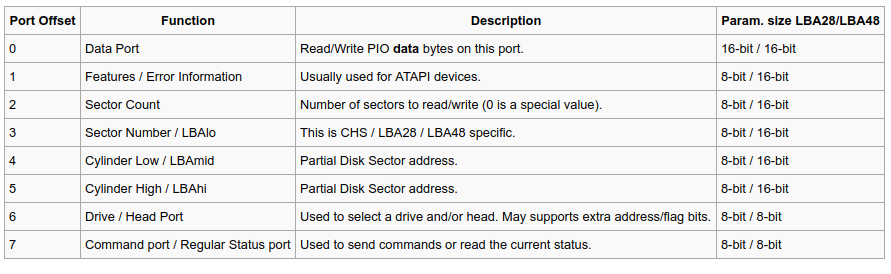
\includegraphics[width=14cm]{pic/assets/ATA_ports}
    \caption{ATA硬盘0x1F0至0x1F7端口的功能}	\label{ATA_ports}	\end{figure}
% \begin{tabular}{|c|c|c|c|}% 通过添加 | 来表示是否需要绘制竖线
%     \toprule
% 	Port Offset& 	Function	& Description	& Param. size LBA28/LBA48\tabularnewline
%     \midrule
% 	0	& Data Port	& Read/Write PIO data bytes on this port.& 	16-bit / 16-bit\tabularnewline
% 	1	& Features / Error Information & 	Usually used for ATAPI devices.& 	8-bit / 16-bit\tabularnewline
% 	2	& Sector Count	& Number of sectors to read/write (0 is a special value).	& 8-bit / 16-bit\tabularnewline
% 	3	& Sector Number / LBAlo	& This is CHS / LBA28 / LBA48 specific.	8-bit / 16-bit\tabularnewline
% 	4	& Cylinder Low / LBAmid & 	Partial Disk Sector address.	& 8-bit / 16-bit\tabularnewline
% 	5	& Cylinder High / LBAhi & 	Partial Disk Sector address.	& 8-bit / 16-bit\tabularnewline
% 	6	& Drive / Head Port	& Used to select a drive and/or head. May supports extra address/flag bits.	& 8-bit / 8-bit\tabularnewline
% 	7	& Command port / Regular Status port & 	Used to send commands or read the current status.	& 8-bit / 8-bit\tabularnewline
%     \bottomrule
% \end{tabular}

硬盘有三种访问模式,一是"CHS mode",即通过柱面(Cylinder)、磁头(Head)、扇区(Sector)来访问,这种方式
相对比较麻烦,而且能访问到的容量有限;二是"LBA28 mode";三是"LBA48 mode".前两种方法已经过时了,用"LBA48 mode"
可以访问更大的容量,而且更为方便,我们采用的是"LBA48 mode".

通过get\_hd\_size(0)和get\_hd\_size(1),我们分别得到了hd1和hd2的硬盘容量.因为我们的文件系统建立在硬盘1(hdb)上,
通过端口,发送命令切换到hdb(switch\_to\_disk(1)).

\subsection{选择IDE(ATA)硬盘}



\subsection{硬盘读写}
这里仅是写,读也类似,使用的是LBA访问方式,由于一次传不了很长的地址,需要把地址拆开成几段,
依次传输,这里需要查阅ATA硬盘的相关资料(推荐到osdev.org查阅).用这种访问磁盘的方式,写出来
都大同小异,只需要符合规范即可.这里确保是针对硬盘1进行读写,存放内核的硬盘0不去动它.

\begin{minted}{c}
void IDE_write_sector(void *src,int lba)
{
	switch_to_disk(1);
	set_disk_no(1);/*disk1 :PC hard disk */
	IDE_disk_wait();
	outb_wait(ATA_PORT_SECT_COUNT,1);/*outb(0x1f2,1);*/
	outb_wait(ATA_PORT_LBA_LOW ,lba);/*outb(0x1f3,lba);*/
	outb_wait(ATA_PORT_LBA_MID ,lba >> 8);/*outb(0x1f4,lba>>8)*/
	outb_wait(ATA_PORT_LBA_HIGH ,lba >> 16);/*outb(0x1f5,lba>>16)*/
	outb_wait(ATA_PORT_DEVICE , 0xe0 |(disk_no&1)<<4| (lba >> 24));/*outb(0x1f5,lba>>16)*/
	/*disk_no determines write to which disk.*/
	outb_wait(ATA_PORT_STATUS, HD_WRITE);
	IDE_disk_wait();
	for(int i = 0; i < SECTOR_SIZE/4 ; i++){
	     _out_data32(ATA_PORT_DATA,((u32*)src)[i]);
	}
}
\end{minted}
\section{建立硬盘分区表}
这里有关于硬盘分区表的简单介绍(http://www.gotothings.com/unix/disk-partition-table.htm).


\section{基于位示图的inode分配与回收}
位示图的方法比较简单.在
\begin{minted}{c}
	int new_inode()
	{
		u8 sector[512]={0};
		int i = 0;rios_superblock.s_startsect = 1;
		IDE_read_sector((void *)&sector,NR_INODE_MAP_BLK(rios_superblock));
		for(i=0;i<512*8;i++){
			if(bitmap_test_bit(i,sector)){
				;
			}else{
				bitmap_set_bit(i,sector);
				IDE_write_sector((void *)&sector,NR_INODE_MAP_BLK(rios_superblock));
				return i;
			}
		}
		return i;
	}
\end{minted}	
\section{建立根目录}
这里要申请inode号并分配数据区,建立"."和"..",如果是初次建立文件系统,
应当把系统中默认的目录如/usr等建立好,创建大文件jane.txt和小文件hamlet.txt
留待测试用.第二次"make run"或"make qemu"进系统时就不需要做这些了.

\section{基于成组链接法的磁盘空闲块管理}
\begin{minted}{c}    
int new_block()
{
	union Super_Block_Sect *p_ri_sb = get_super();
	set_super();
	if(!is_specific_block_set){
/*initially, the first( counting from 1 ) data block is allocated for specific block.*/		
		p_ri_sb->s_specific_blk_nr = 1;set_super();/*write back to disk*/
		specific_block = get_blk_nr_free_group(p_ri_sb->s_specific_blk_nr);
		is_specific_block_set = 1;
	}
/* remember to write back to disk. */	
again:	
	if(specific_block.s_free > 1){
		specific_block.s_free --;
		set_specific_blk_nr(p_ri_sb->s_specific_blk_nr);/*write back*/
		set_blk_nr_free_group(specific_block,p_ri_sb->s_specific_blk_nr);
		return specific_block.s_free_blk_nr[specific_block.s_free];
	}else if(specific_block.s_free == 1){
		specific_block.s_free --;
		int current_group_nr = p_ri_sb->s_specific_blk_nr;
		int next_group_nr = specific_block.s_free_blk_nr[0];
/* get NR of next group,copy its contents to specific block in memory through buffer
 * , and **allocate current block**. 
 */
		specific_block = get_blk_nr_free_group(next_group_nr);
		set_specific_blk_nr(next_group_nr);
/* now, we are switching to a different specific block*/		
		specific_block.s_free --;
/* XX return specific_block.s_free_blk_nr[specific_block.s_free];
 * ok,we were able to return NR here,but in that case,the following code won't execute,
 * and the last specific block haven't been allocated.
 */		
		int tmp = specific_block.s_free_blk_nr[specific_block.s_free];
		{/* allocate the last specific block */
			specific_block.s_free_blk_nr[specific_block.s_free] = current_group_nr; 
			specific_block.s_free ++; 
		}
		if(tmp!=0){
/*write back*/
			set_blk_nr_free_group(specific_block,p_ri_sb->s_specific_blk_nr);
			return tmp;
		}else{/*SHOULD NOT allocate root*/
			goto again;
		}
	}else if(specific_block.s_free == 0){
		_panic(" FBI WARNING:There is no free block available!!!");
	}	
}
\end{minted}
\section{超级块设计}
超级块的s\_magic为rifs文件系统的魔幻数字,这里我设其为0x88,开机时若在磁盘上
超级块对应位置探测到0x88,系统就认为已经安装rifs文件系统.以下为磁盘超级块结构.

\subsection{硬盘超级块}
\begin{minted}{c}    
struct d_super_block
{
u16 s_ninodes;
u16 s_capacity_blks;/*capacity count in blocks*/
u16 s_startsect;/*超级块的起始扇区,sector0为boot sector,故超级块从1开始*/
u16 s_zone_bitmap_blks;/*according to Prof Jiang,we will not use this policy (data block bitmap) anymore.*/
u16 s_inode_bitmap_blks;/*num of blks that bitmap takes up*/
u16 s_inode_blks;
u16 s_firstdatazone;
u16 s_specific_blk_nr_group;/*成组链接专用块对应磁盘上的组号*/
u16 s_magic;/*ri_fs magic:0x88*/
};    
\end{minted}

\section{inode设计}
\subsection{内存中inode结构(m\_inode)}
\begin{minted}{c}   
struct m_inode
{
	u8 i_mode;			/*file type(dir/normal) and attribute(rwx)*/
	u8 i_uid;			/*user id*/
	u8 i_gid;			/*group id*/
	u8 i_nlinks;			/*num of files that link to it*/
	u8 padding0[2];
	u32 i_creat_time;	
	u16 i_zone[10];
	u16 i_ino;			/*inode id号 (bitmap)*/
	u32 i_size;			/*size of file*/
	u32 padding1[7];		/*占位 8*32个字节*/
/* ok,let's make sizeof(d_inode) exactly equal to 64,that's 512bits,
 * a sector can put exactly 8 of d_inode.
 * if we attemp to extend the m_inode and d_inode,make sure that
 * they are in sync with each other,and adjust the fields and paddings
 * without changing the sizeof(d_inode)
 * zone[0~6]:	direct block 
 * zone[7]:	single indirect block
 * zone[8]:	double indirect block 
 * zone[9]:	trible indirect block
 *These are only in memeory*/
	u32 i_access_time;
	u8 i_mount;
	u8 i_dev;			/*hd0 or hd1*/
	u8 i_dirty;
	u8 i_updated;
	u8 i_count;			/*引用数*/
	struct task_struct *i_wait;	/*not implemented yet*/
}__attribute__((packed));		/*一定要加,不然字节对不齐,会多用空间*/
\end{minted}

请控制好d\_inode的大小以及与m\_inode同步性.这里设置几个padding的意义在于占位,
我把d\_inode 的大小控制在8*6+32+16*10+16+32*8=512 bits,这样一个扇区512*8=4096bits,
正好可以放8个d\_inode,尽量避免跨扇区操作inode.

磁盘inode和内存inode的数据结构上相似,即内容上磁盘inode结构是内存inode结构的子集,
内存inode不但要保存磁盘inode的所有信息,还要保存进程和系统运行中的相关信息.为避免操纵磁盘inode时跨扇区操作,
这里我严格控制d\_inode结构体的大小,为512bits,即64B,而一个扇区512B,恰好可以放8个磁盘inode,
这里attribute((packed))很重要,如果不加的话,编译器为了字节对齐,一个结构体将使用多于64B的空间,
这样将导致inode的存放很碎,操作出问题.机构体里的padding主要是为了占位,凑到恰好64B,日后若扩展d\_inode时,
就减少padding的数量,然后加上要增加的新项,保持sizeof(struct d\_inode)不变.

\subsection{iget和iput}
内存中有inode的拷贝,iget和iput功能就是从硬盘上拷贝inode到指定内存或把内存中inode拷到硬盘.
有时会出现"脏数据"的情况,所以要特别注意内存与硬盘上信息的同步,不要忘记写回.

\section{目录管理}

\subsection{列出目录(ls)}
显示当前路径下有什么.

\subsection{创建和删除目录(mkdir、rmdir)}

有了在当前目录创建一级目录的基本操作以后,名字的分割是创建多级目录的关键,
比如要递归创建"dir1/dir2/dir3",要如何依次分解出dir1、dir2、dir3呢?
C标准库中解决这个问题对应着一个函数strtok,在string.h中.strtok该函数返回
被分解的最后一个子字符串,如果没有可检索的字符串,则返回一个空指针。string.h
中strtok的实现并不长,然而十分高效,也具有鲁棒性.要我写出这个函数是不出来的
,我们也不需要彻底重复制造轮子,那就借用一下库函数string.h的实现吧.这里函数
\mintinline{c}!char * strtok(char * s,const char * ct)!一共18行代码,
源于Linux2.4/lib/string.c,特此说明.

\begin{minted}{c} 
char *strtok(char s[], const char *delim);
//库函数strtok用法:分解字符串为一组字符串。s为要分解的字符串,delim为分隔符字符串。
\end{minted}

根据里奇的"KISS"懒汉原则,我把目录管理和文件管理的函数做到尽量傻瓜,比如mkdir函数只
支持在当前目录创建目录,至于多级目录的创建,则通过其他函数分解字符串,拆出各个单级目录
名,分别调用mkdir函数来实现mkdir dir1/dir2/dir3这样的功能,其他诸如cd dir1/dir2/dir3
也类似,不再重复说明.

在本系统中,不允许在同一目录创建同名文件夹.创建目录首先给目录分配inode和数据区,由于一个目录项所占空间是一定的,
故可以通过一个目录的大小除以目录项的大小得到目录的总数.

目录名长度有效,超过长度就报错.创建一个新目录时,应当先首先给它添加两个目录项指向自身的"."和父目录"..",
然后更新目录的大小.写回到磁盘.

删除目录也类似,要归还数据区和inode号.不过当要删除的目录不为空的情况下,不允许删除目录的操作.

\subsection{hexdump}
在DOS下学习汇编时会有以十六进制查看一块数据区的情况,Linux中也有类似的hexdump命令.
为了方便调试,更方便地找出问题,本系统也提供简单的hexdump命令,只提供最基本的功能.

图~\ref{hexdump523}~展示了硬盘1的第523扇区的内容.
\begin{figure}[!htbp]
    \centering	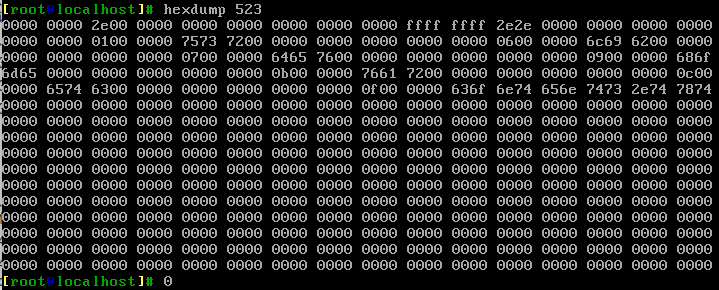
\includegraphics[width=14cm]{pic/assets/hexdump523}
	\caption{hexdump523}	\label{hexdump523}	\end{figure}
	
可以看到出现了十六进制的2e,不远处还有连续的两个2e,通过man ascii命令查ASCII码表可知这是"."和
"..".因此这是一个目录的数据区.

图~\ref{wxHexEditor}~是用wxHexEditor软件查看rios/build/hd.img的磁盘镜像.
\begin{figure}[!htbp]
    \centering	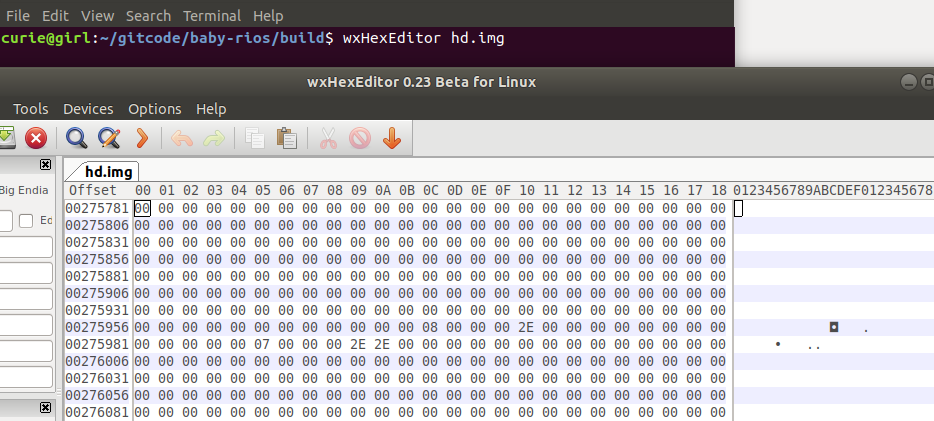
\includegraphics[width=14cm]{pic/assets/wxHexEditor}
	\caption{wxHexEditor}	\label{wxHexEditor}	\end{figure}
	
利用虚拟机编写测试时,我们也可以通过sublime软件打开rios/build/hd.img文件,这样直接
观测到"硬盘"上的数,可以与我们在系统中"hexdump 扇区号"得到的结果相比对,以验证hexdump的正确性. 
	
\subsection{切换目录(cd)}
支持多级切换,如cd dir1/dir2/dir3.多级的原理也是分解路径,和mkdir类似.

\paragraph{查看当前目录(pwd)}

使用pwd命令


\section{文件管理}
这里有三个关键的表,有:主存活动inode表、系统打开文件表、用户打开文件表.
他们的结构如下.

1.活动inode表.
\begin{minted}{c}
	struct active_inode_table{
		struct m_inode inode_table[MAX_ACTIVE_INODE];
	};   
\end{minted}

2.系统打开文件表:

\begin{minted}{c}
struct file file_table[NR_FILE];	   
\end{minted}

文件表整个系统中只有1张。该表可以视为结构体数组.

3.用户打开文件表(下面其中一个数据项):

进程控制块task\_struct
\begin{minted}{c}
	struct task_struct{
		u8 gid;
		u8 uid;
		struct m_inode * pwd;
		struct m_inode * root;
		struct file * filp[NR_OPEN];	/* 进程表项 */
	/* this is user-wide file table */	
	};	   
\end{minted}

理论上应该包含于进程PCB之中,每个进程有一份.

进程PCB记录当前的组id和用户id,内存inode指针pwd指向当前目录的inode,
内存inode指针指向当前根目录的inode,进程表项\mintinline{c}!struct file * filp[NR_OPEN]!,
为用户打开文件表.

由于工作量的问题,我没有做进程管理,但是为了可扩展性,还是定义了task\_struct,
用户打开文件表是进程表项,对应task\_struct里的\mintinline{c}!struct file * filp[NR_OPEN]!
.文件描述符表,每个进程有且仅有1张。该表可以视为指针数组,数组的元素指向文件表的一个元素。
最重要的是:数组元素的下标就是文件描述符。

这三个表中,活动inode表从磁盘上拷贝inode,另外由于表中结构体是struct m\_inode,
还存一些系统运行时的相关信息,比如内存m\_inode中的i\_count即被引用次数.
系统打开文件表file\_table其表中项的结构是file,file中包含指向m\_inode的指针,
即指向活动inode表的表项.用户打开文件表filp[NR\_OPEN],其中表项的结构是* file,即文件的指针.
文件描述符fd是filp[..]指针数组的index下标,fd可以看做file索引的索引.



\subsection{文件的打开和关闭}

\paragraph{文件结构} file:

\begin{minted}{c}
	struct file
	{
		u8 f_mode;			        /*文件读写模式及权限管理*/
		u8 f_flags;
		u16 f_count;			    /*file引用次数*/
		struct m_inode * f_inode;	/*指向活动inode表中文件的inode*/
		u32 f_pos;
	};	
\end{minted}

\paragraph{目录项结构} dir\_entry

\begin{minted}{c}
struct dir_entry{
	u32 inode;
	u8 name[MAX_NAME_LEN];
}__attribute__((packed));
\end{minted}


这里目录项对应目录中的一条记录的结构,记录两项内容,一是inode号,二是文件或目录名字.

\subsection{open}
open函数的功能是:给它输入文件名,然后返回有效的文件描述符.
首先按名查找,在当前目录根据文件名找到要打开的文件的inode号,
新建一个i节点表元素,让其对应打开的物理文件(如果对应于该物理
文件的i节点元素已经建立,就不做任何操作);

让其指向刚建立的文件表元素。最后将该元素的下标作为open的返回值返回。

这样当调用read(write)时,根据传入的文件描述符,操作系统就可以找到对应
的文件描述符表元素,进而找到文件表的元素,进而找到i节点表元素,从而完成对物理文件
的读写。




\begin{minted}{c}   
int open(const char *name){
	int fd,i;
	int ino = get_dir((char *)name);
	if(ino==0){
		kprintf(" open:failed, ino cannot be zero.");
		return -1;
	}
	if(ino==-1){
		kprintf("\n open: '%s':no such file or directory.",name);
		return -1;
	}
/* search the active inode table, if it's not in this table,just copy.*/	
	for(i=0;i<MAX_ACTIVE_INODE;i++){
		if(active_inode_table.inode_table[i].i_ino == ino)
			break;
	}
	int active_inode_table_nr=get_active_inode_table_nr();
	if(i>=MAX_ACTIVE_INODE){/*no record found,need to copy. */
		if(active_inode_table_nr>MAX_ACTIVE_INODE)_panic("FBI_WARNING:CAN NOT open more than 64 files at the same time!");
		iget(&active_inode_table.inode_table[active_inode_table_nr],ino);

	}else{/* it has been opened before, no nead to copy */
	      /* here,we get i */
		if(current->filp[i]->f_inode->i_ino == ino)return i;
		goto comeon;
	}
comeon:	
/* find a blank entry in process's file descriptor table */	
	for(fd=0 ; fd <NR_OPEN ; fd++ ){

		if(!current->filp[fd])
			break;
	}
	if(fd>=NR_OPEN)
		return -1;/* overflow */
/* find a blank entry in system file table */	
	file * p_ft = file_table;
	int j;
	for(j=0;j<NR_FILE;j++,p_ft++){
		if(!p_ft->f_count) break;
	}
	if(j>=NR_FILE){
		kprintf("\n failed to create.");
		return -1;
	}
	int valid_file_table_nr = j;
/* ok, let filp[fd] points to a entry in file table,and let f_count+=1 */
(current->filp[fd]=p_ft)->f_count++;
/* NOTICE! here we should let filp[fd]->f_inode point to an entry in active_inode_table*/
current->filp[fd]->f_inode = &active_inode_table.inode_table[active_inode_table_nr];
/* keep there tables in sync with each other */
	return fd;
}
\end{minted}

\subsection{多级索引}

系统中jane.txt这个文本文件有几MB大小,装下了《Jane Eyre》这部英文小说的全部内容,
大小足够测试了.

用cat jane.txt可以成功显示全书内容.如图~\ref{cat_jane}~所示

\begin{figure}[!htbp]
	\centering	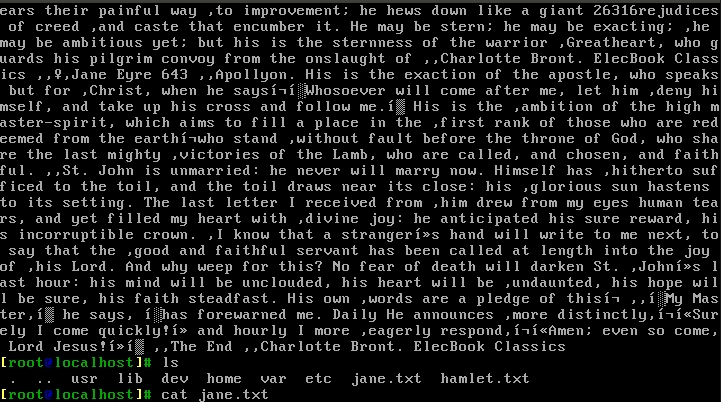
\includegraphics[width=14cm]{pic/assets/cat_jane}
	\caption{用cat命令查看jane.txt文本文件内容}	\label{cat_jane}	\end{figure}

cat显示命令比较快,一分钟之内可以把整本书的内容输出.用slowcat jane.txt也可以显示全书内容,
但速度很慢.如图~\ref{cat_jane}~所示.	

\begin{figure}[!htbp]
		\centering	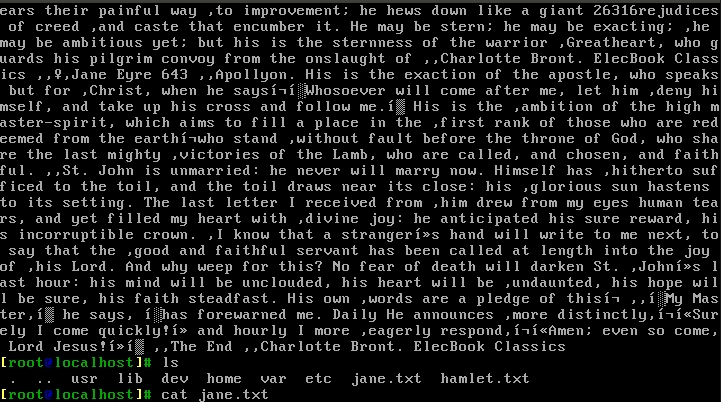
\includegraphics[width=14cm]{pic/assets/cat_jane}
		\caption{用slowcat命令查看jane.txt文本文件内容}	\label{cat_jane}	\end{figure}

\subsection{读写文件与删除文件}

由于是多级索引,删除文件实现起来比较麻烦,这里留到关键函数实现中谈.

\subsection{查看文件内容(cat)}

如图~\ref{cat_hamlet}~所示

\begin{figure}[!htbp]
	\centering	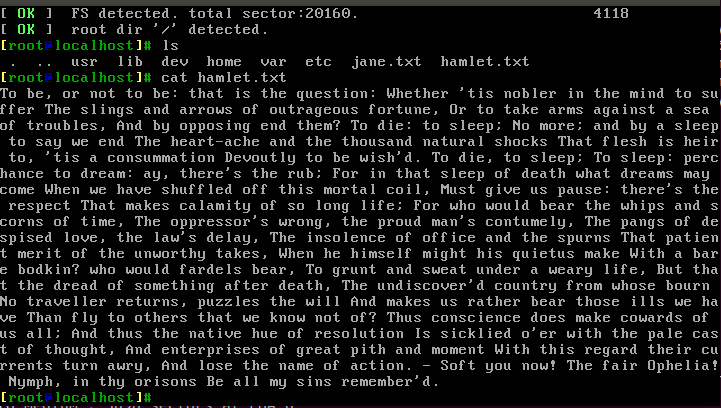
\includegraphics[width=14cm]{pic/assets/cat_hamlet}
    \caption{用cat命令查看文本文件内容}	\label{cat_hamlet}	\end{figure}

\subsection{查看硬盘1结构组成}
用自定义命令info disk查看,硬盘1由引导扇区(我们的内核在硬盘0,这里作用不大)、超级块、
废弃的数据区位示图区、inode区和数据区组成.本来准备使用位示图完成数据区的空闲空间管理
,后来应老师要求,改为成组链接方式,因而数据区的位示图区废弃不用.关于系统中命令的用法,
可通过help命令查看.

硬盘1结构组成如图~\ref{disk}~所示.

\begin{figure}[!htbp]
	\centering	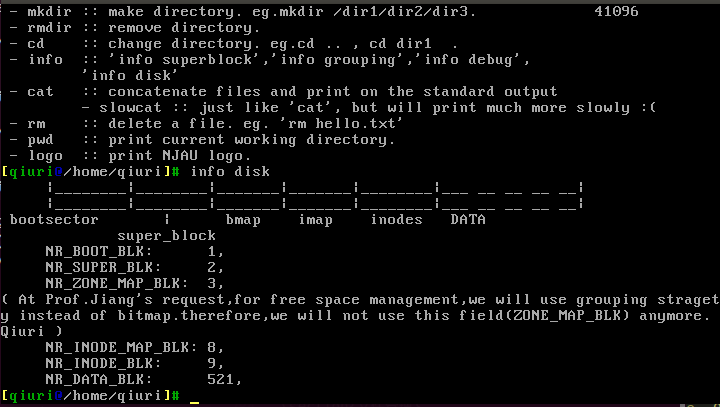
\includegraphics[width=14cm]{pic/assets/disk}
    \caption{硬盘1结构组成}	\label{disk}	\end{figure}








% \clearpage
 

\chapter{软件系统设计} 
% \pagenumbering{arabic} % 阿拉伯数字页码
% 包括系统类图、顺序图等。论述软件系统结构、所完成功能的具体实现流程,对应类、方法函数等,可用伪码并论述
模块功能大致是这样:src/kernel处理系统中异常、中断及调度等核心功能;blk\_dev为字符设备驱动,
处理ATA(也叫IDE)硬盘驱动,硬盘分区表的检测和写入等,完成了设备管理,为文件系统的实现提供基础;
mm是内存管理,这里采用相对比较简单的连续内存分配;include文件夹下面是各个c++源文件的头文件,
包括一些重要的宏定义以及对部分x86指令向上层的封装;fs为文件系统主要模块,完成了inode的位图分配回收
和数据块的成组链接分配回收、超级块的管理、用户打开文件表和系统打开文件表及活动inode表之间的联系和管理等;
app模块包括但不限于文件系统的一些命令的实现如mkdir、pwd、ls、touch、rmdir等的函数实现.


依赖关系如图~\ref{dependency_graph}~所示.	

\begin{figure}[!htbp]
		\centering	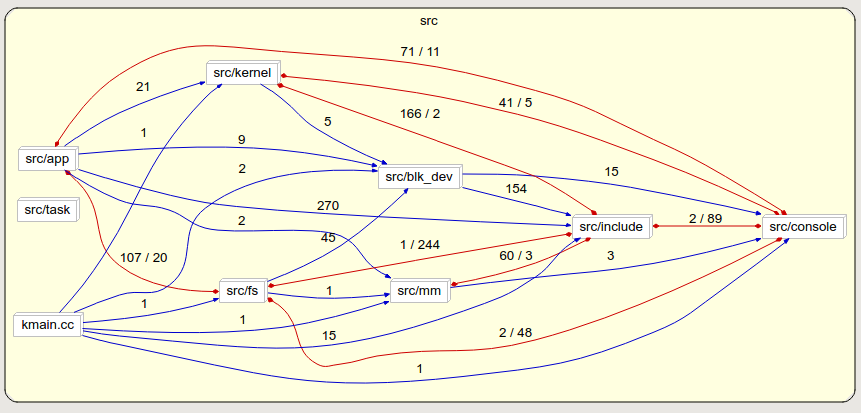
\includegraphics[width=14cm]{pic/assets/dependency_graph}
		\caption{RiOS内核依赖关系图}	\label{dependency_graph}	\end{figure}


目录结构如图~\ref{directory_structure}~所示.	

     \begin{figure}[!htbp]
            \centering	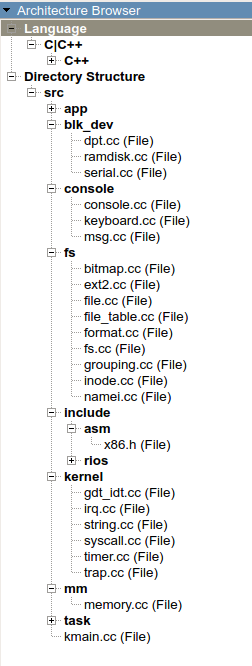
\includegraphics[width=9cm]{pic/assets/directory_structure}
            \caption{目录结构图}	\label{directory_structure}	\end{figure}

\section{系统类图}            

UML类图1如图~\ref{UML_1}~所示.	

     \begin{figure}[!htbp]
            \centering	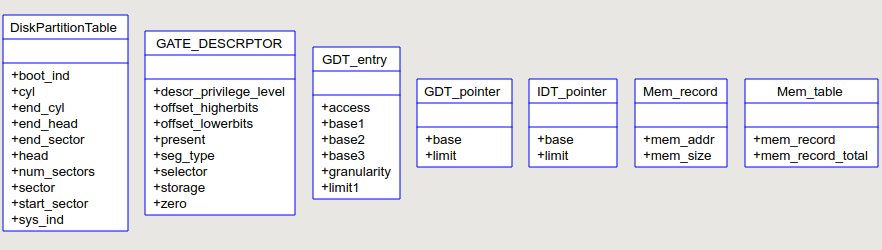
\includegraphics[width=14cm]{pic/assets/UML_1}
            \caption{UML Class Diagram(1) of RiOS kernel}	\label{UML_1}	\end{figure}

UML类图2如图~\ref{UML_2}~所示.	

     \begin{figure}[!htbp]
            \centering	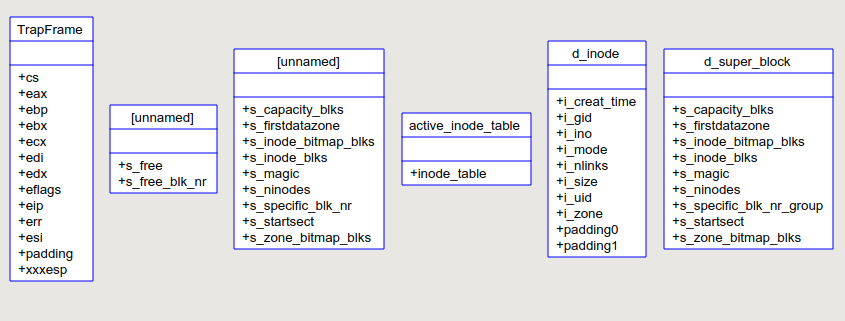
\includegraphics[width=14cm]{pic/assets/UML_2}
            \caption{UML Class Diagram(2) of RiOS kernel}	\label{UML_2}	\end{figure}

UML类图3如图~\ref{UML_3}~所示.	

     \begin{figure}[!htbp]
            \centering	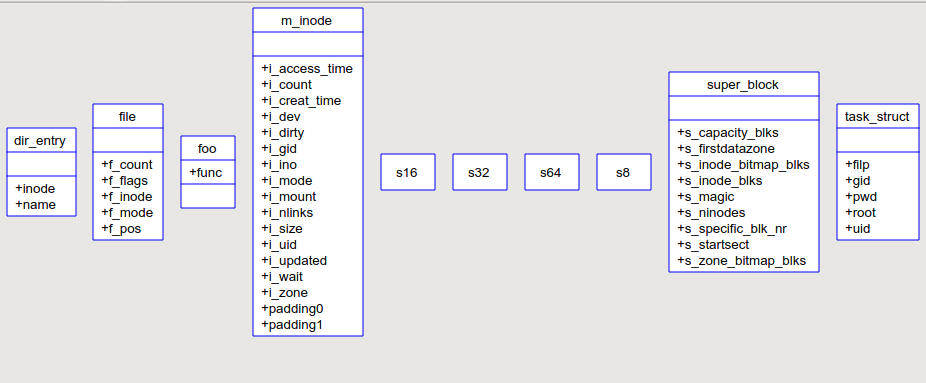
\includegraphics[width=14cm]{pic/assets/UML_3}
            \caption{UML Class Diagram(3) of RiOS kernel}	\label{UML_3}	\end{figure}            

\section{顺序图}
这里展示了开机后做的一系列工作.
顺序图如图~\ref{sequential}~所示.	

     \begin{figure}[!htbp]
            \centering	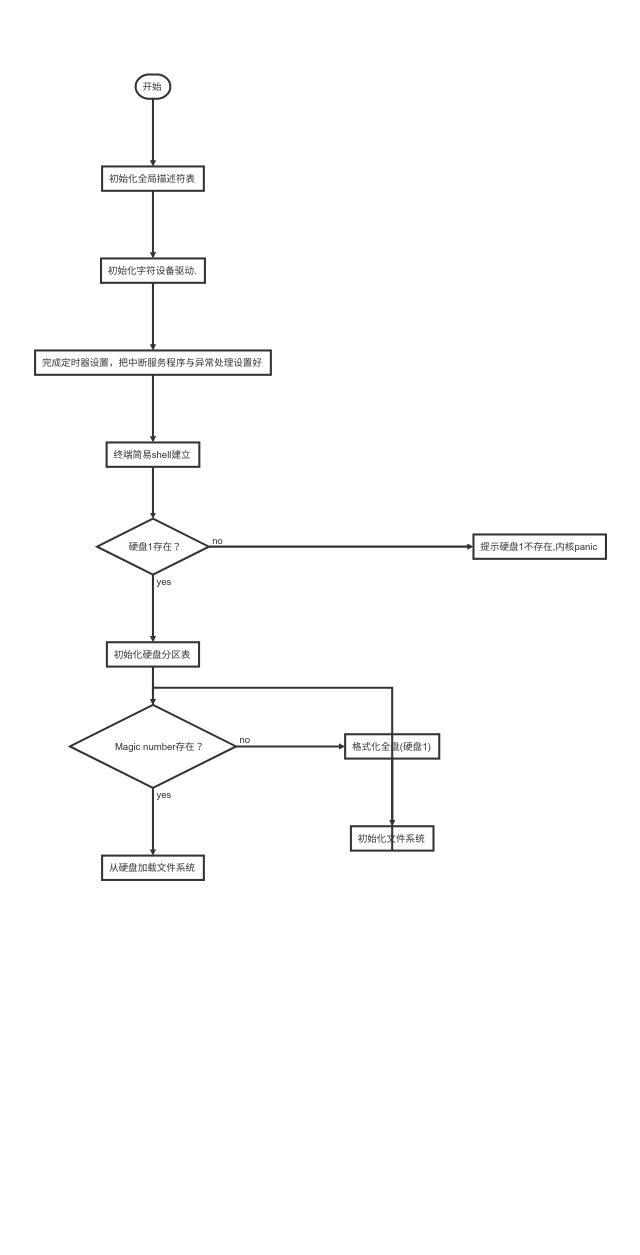
\includegraphics[width=14cm]{pic/assets/sequential}
            \caption{顺序图}	\label{sequential}	\end{figure} 

\section{组成}

\subsection{整体组成}
整体组成如图~\ref{ArchitectureGraph-src}~所示.	

\begin{figure}[!htbp]
       \centering	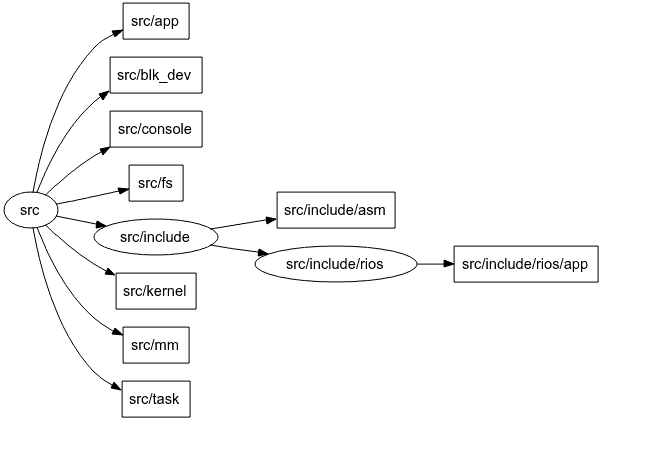
\includegraphics[width=14cm]{pic/assets/ArchitectureGraph-src}
       \caption{ArchitectureGraph-src}	\label{ArchitectureGraph-src}	\end{figure} 

如图~\ref{rios_treemap}~所示.	

     \begin{figure}[!htbp]
            \centering	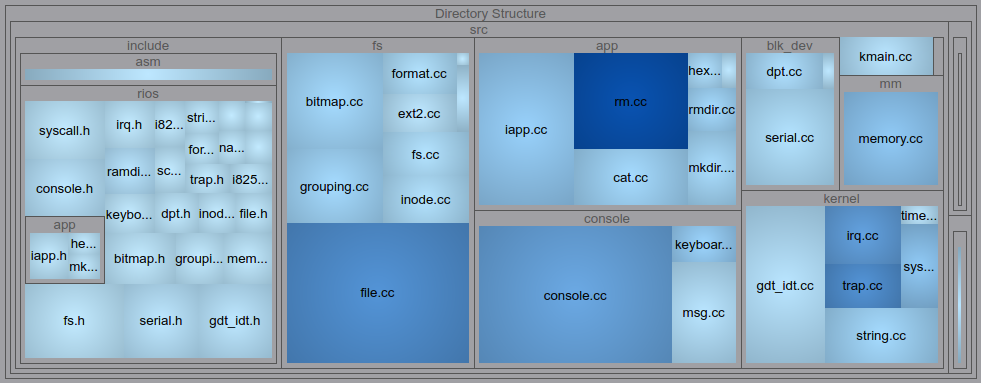
\includegraphics[width=14cm]{pic/assets/rios_treemap}
            \caption{rios treemap}	\label{rios_treemap}	\end{figure} 

\subsection{文件系统组成}
文件系统部分如图~\ref{fs_treemap}~所示.	

     \begin{figure}[!htbp]
            \centering	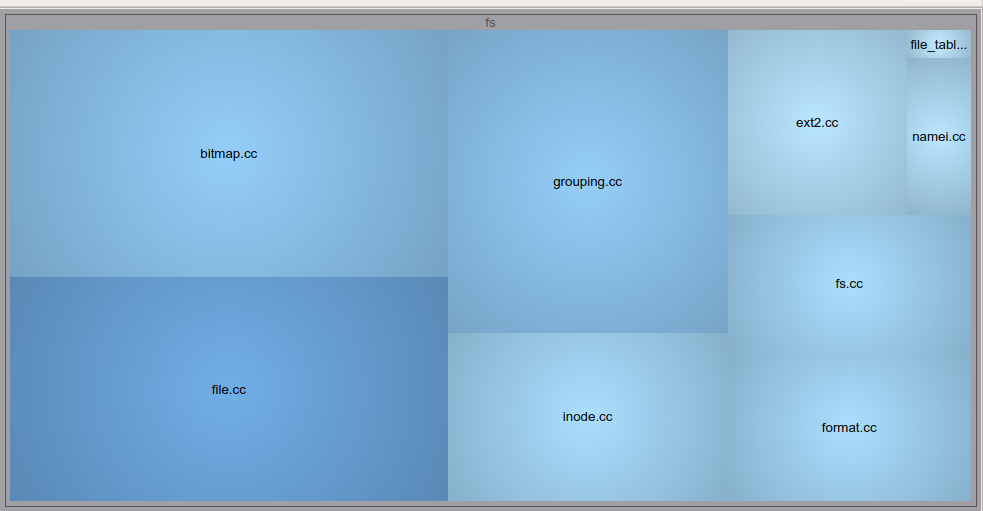
\includegraphics[width=14cm]{pic/assets/fs_treemap}
            \caption{fs treemap}	\label{fs_treemap}	\end{figure} 

\section{依赖关系图}

\subsection{file.cc的依赖关系图}
file.cc依赖关系1如图~\ref{ButterflyGraph-file-cc}~所示.	

     \begin{figure}[!htbp]
            \centering	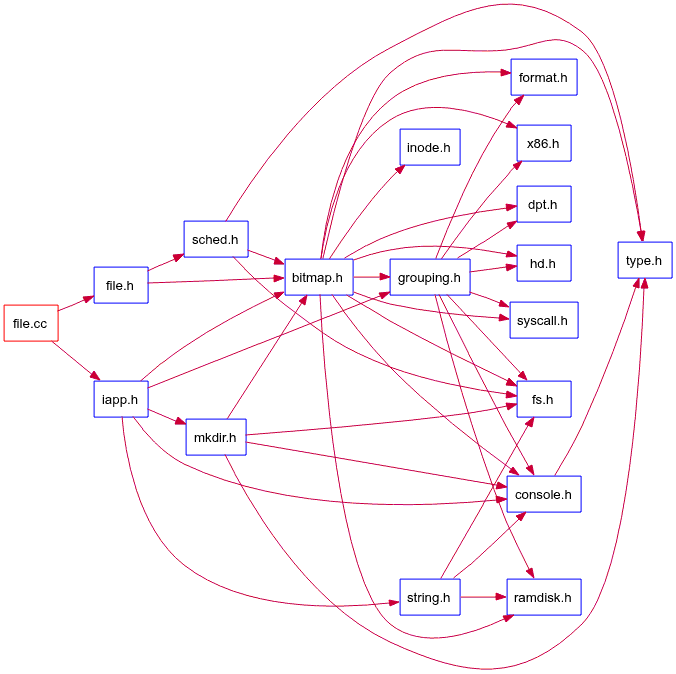
\includegraphics[width=14cm]{pic/assets/ButterflyGraph-file-cc}
            \caption{ButterflyGraph-file-cc}	\label{ButterflyGraph-file-cc}	\end{figure} 
          

\subsection{fs.cc的依赖关系图}
file.cc依赖关系1如图~\ref{ButterflyGraph-fs-cc}~所示.	

     \begin{figure}[!htbp]
            \centering	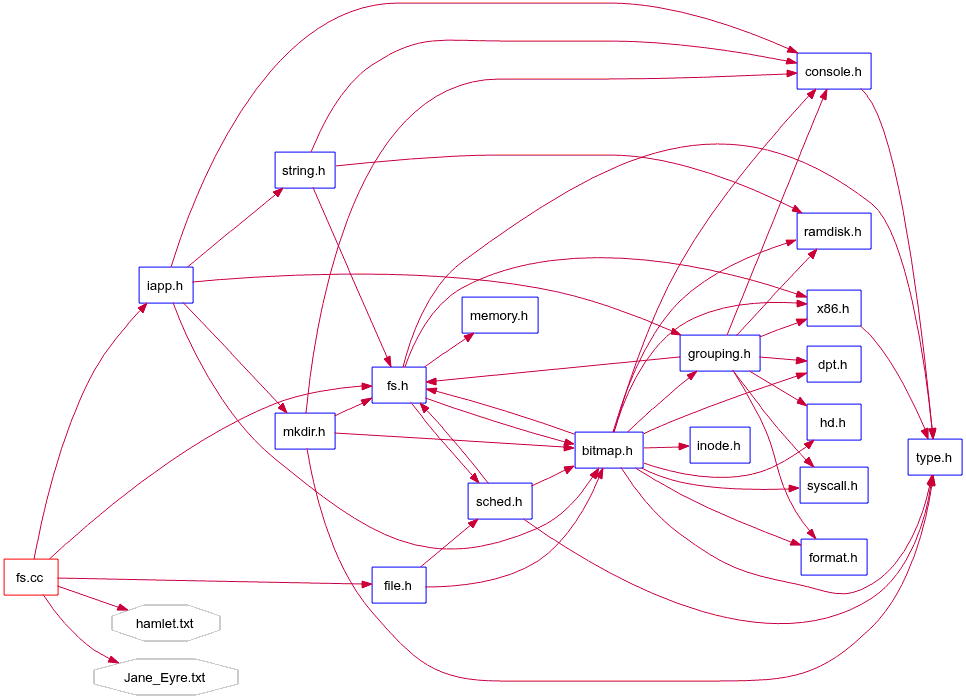
\includegraphics[width=14cm]{pic/assets/ButterflyGraph-fs-cc}
            \caption{ButterflyGraph-fs-cc}	\label{ButterflyGraph-fs-cc}	\end{figure} 

这里只对file.cc和fs.cc两个代码文件依赖关系进行分析,其他可借助understand源代码阅读软件来分析RiOS代码.            

\subsection{整体内部依赖关系图}


整体上,kmain.cc依赖关系1如图~\ref{ButterflyGraph-kmain-cc}~所示.	

     \begin{figure}[!htbp]
            \centering	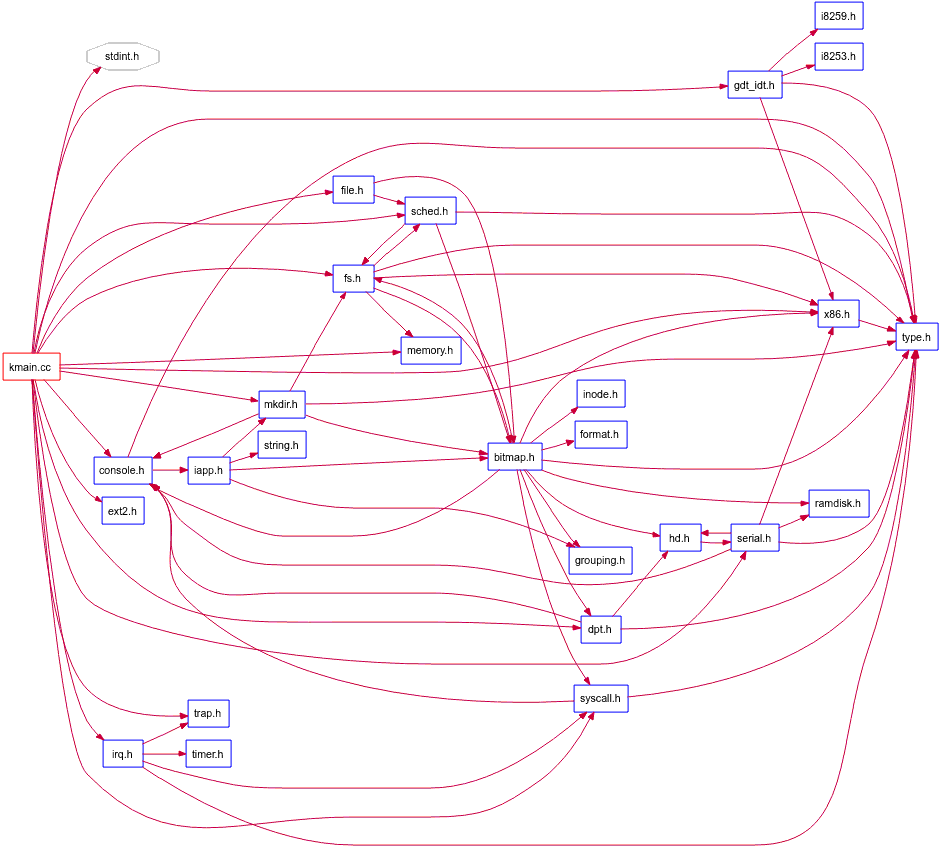
\includegraphics[width=14cm]{pic/assets/ButterflyGraph-kmain-cc}
            \caption{ButterflyGraph-kmain-cc}	\label{ButterflyGraph-kmain-cc}	\end{figure} 


内部依赖图1如图~\ref{ArchInternalDependencies-DirectoryStructure}~所示.	

     \begin{figure}[!htbp]
            \centering	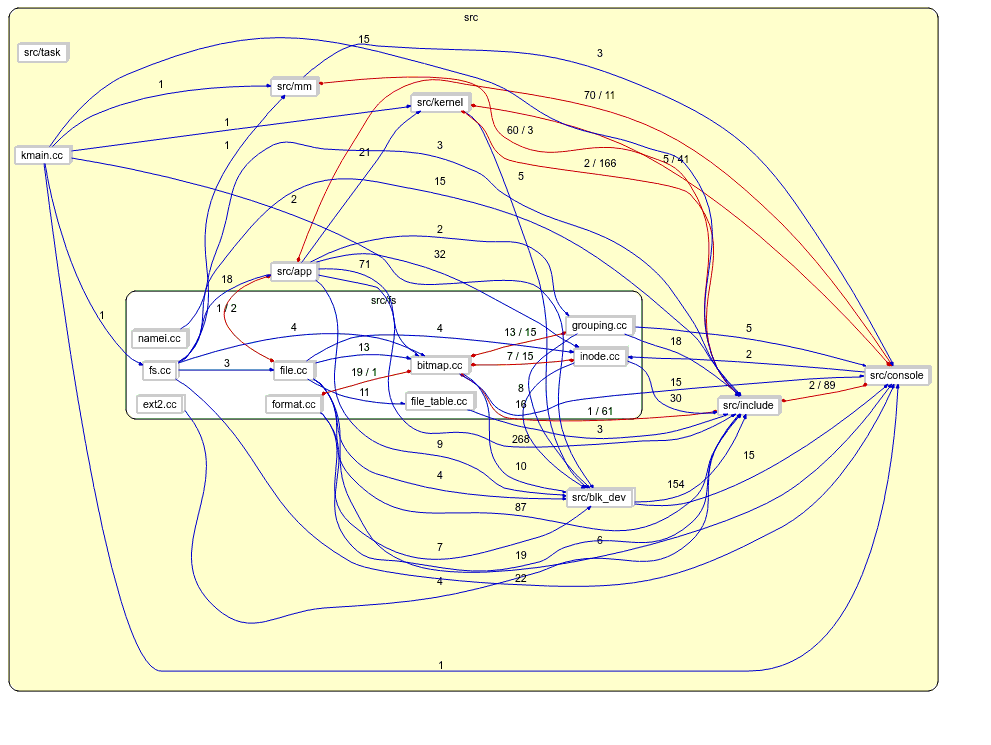
\includegraphics[width=14cm]{pic/assets/ArchInternalDependencies-DirectoryStructure}
            \caption{内部依赖图1}	\label{ArchInternalDependencies-DirectoryStructure}	\end{figure} 

内部依赖图2如图~\ref{ArchInternalDependencies-DirectoryStructure2}~所示.	

     \begin{figure}[!htbp]
            \centering	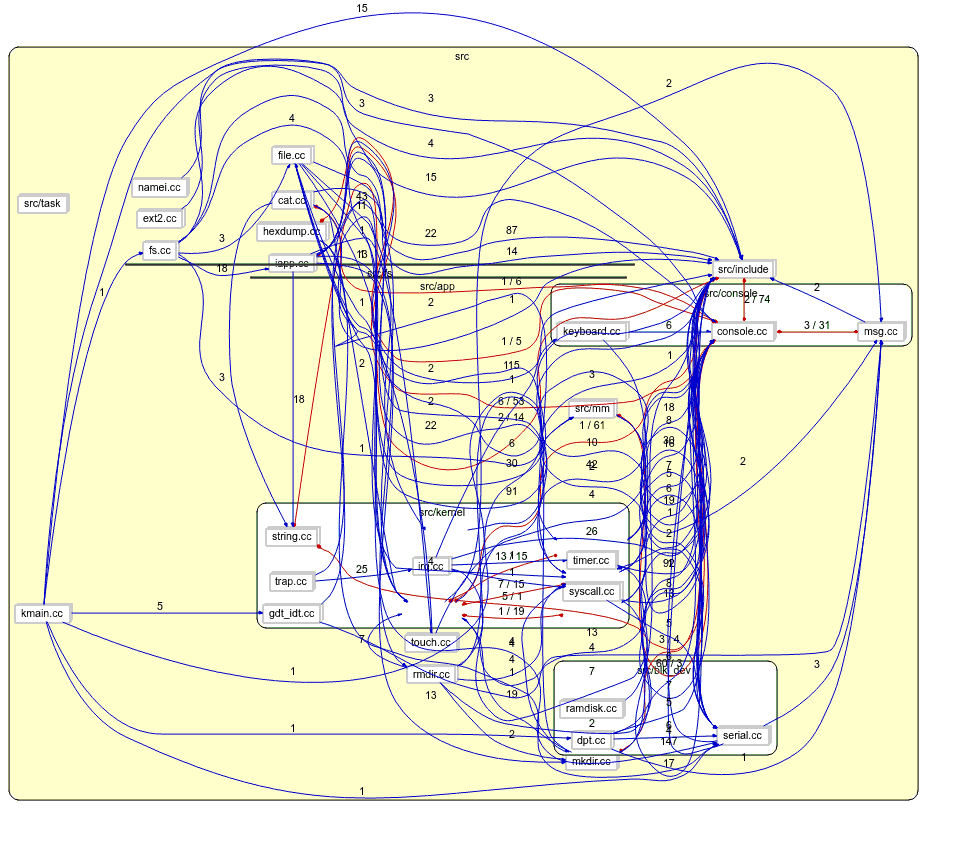
\includegraphics[width=14cm]{pic/assets/ArchInternalDependencies-DirectoryStructure2}
            \caption{内部依赖图2}	\label{ArchInternalDependencies-DirectoryStructure2}	\end{figure} 

内部依赖图3如图~\ref{ArchInternalDependencies-DirectoryStructure3}~所示.	

     \begin{figure}[!htbp]
            \centering	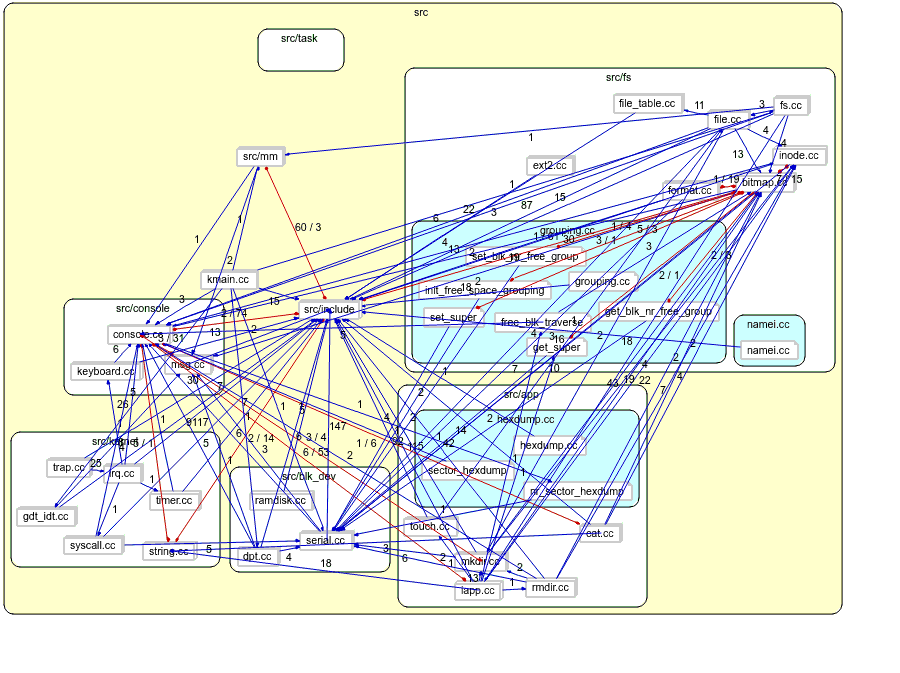
\includegraphics[width=14cm]{pic/assets/ArchInternalDependencies-DirectoryStructure3}
            \caption{内部依赖图3}	\label{ArchInternalDependencies-DirectoryStructure3}	\end{figure} 


% \clearpage 

\chapter{关键操作(方法)函数的实现} 
% \pagenumbering{arabic} % 阿拉伯数字页码
% 与第五部分有所对应,用带注释伪码论述
% 一些例子,可以模仿。

\section{GDT与IDT表项的设置}
GDT和IDT的设置还是相对还是比较复杂的,因为这很大程度上是由x86硬件决定的,
个人不能自由发挥,需要查阅相关手册,了解硬件设计的结构,依此来编写代码.
更麻烦的是,由于x86要考虑兼容性,一些本来简单的几个数据项能要拆成几段,"身首异处",
这就需要我们在设置的时候大量采用位操作,把数据项该拆的拆,该还原的还原,放到他们应放的地方去.
这部分建议阅读赵炯《Linux内核完全剖析》以及osdev网站上有关x86硬件的介绍,维基百科上亦有相关资料
(https://en.wikipedia.org/wiki/Global\_Descriptor\_Table).
\subsection{GDT}
GDT表项高32位如下,granularity粒度位G这里设为1,AVL为系统可用位.

\begin{tabular}{|c|c|c|c|c|}% 通过添加 | 来表示是否需要绘制竖线
    % \toprule
    % Exception \# & Description & Error Code?\tabularnewline
    \midrule
    23 & 22 & 21 & 20 & 19 - 16\tabularnewline
    G  &D/B & L  &AVL & 段界限 \tabularnewline
    1  &1   & 0  &   &        \tabularnewline
    \bottomrule
\end{tabular}

赵炯《Linux内核完全剖析》P91 数据段和代码段在TYPE段的不同编码:


\begin{tabular}{|c|c|c|c|c|}% 通过添加 | 来表示是否需要绘制竖线
    % \toprule
    % Exception \# & Description & Error Code?\tabularnewline
    \midrule
         &        &    &<-  TYPE ->& \tabularnewline 		
     15 & 14-13  & 12 &   11 - 8   & 7 - 0\tabularnewline     
    \bottomrule
\end{tabular}


\begin{tabular}{|c|c|c|c|c|}% 通过添加 | 来表示是否需要绘制竖线
    % \toprule
    % Exception \# & Description & Error Code?\tabularnewline
    \midrule
    data segment:& p &  DPL  & 1 & 0 E W A   \tabularnewline 
    code segment:& p &  DPL  & 1 & 1 C R A   \tabularnewline    
    \bottomrule
\end{tabular}


其中一些字母的含义为: 

E:扩展方向,W:可写,A:已访问,C:一致代码段,R:可读

这部分原理理解起来不是很困难,然而要保证一个位都不能错,否则系统还是不会正常工作,
在位操作的过程中我们可能弄晕了,忘了它本来面目是什么,网站https://wiki.osdev.org/GDT\_Tutorial
提供了一个简单的小程序,我们通过它可以事先算出GDT设置好后是什么样,可以和我们自己用位操作搞出来的GDT
表项的值相互验证,例如运行在ring0和ring3的代码段和数据段应该怎样设置:

\begin{tabular}{|c|c|}% 通过添加 | 来表示是否需要绘制竖线
    \toprule
    值 & 含义\tabularnewline
    \midrule
    0x0000000000000000 & NULL \tabularnewline 
    0x00CF9A000000FFFF & GDT CODE PL0 \tabularnewline 
    0x00CF92000000FFFF & GDT DATA PL0 \tabularnewline 
    0x00CFFA000000FFFF & GDT CODE PL3 \tabularnewline 
    0x00CFF2000000FFFF & GDT CODE PL3 \tabularnewline  
    \bottomrule
\end{tabular}

\subsection{IDT}
IDT表项的设置也应该依据IDT结构图来进行相关位操作,下面是如何把对应的值设置到中断门描述符的操作过程,
陷阱门描述符的设置也与之类似.
\begin{minted}{c}
void set_interrupt_gate(struct GATE_DESCRPTOR *descr, u16 index ,u32 offset, u8 dpl)
{
descr->offset_lowerbits = offset & 0xffff;
descr->selector = index << 3;/*the lower 3 bits is TI(2) and RPI(0,1)*/
descr->zero = 0x00;
descr->seg_type = Gate_INTERRUPT_TYPE;/*0x0E*/
descr->storage = 0b0;
descr->descr_privilege_level = dpl;
descr->present =0b1;
descr->offset_higherbits = (offset & 0xffff0000) >> 16;
}
\end{minted}


\section{成组链接}

\begin{figure}[!htbp]
		\centering	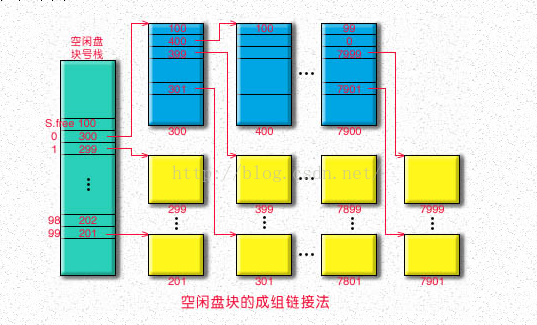
\includegraphics[width=14cm]{pic/assets/grouping}
		\caption{成组链接原理}	\label{grouping}	\end{figure}
		
初始化时,若之前未初始化,先指定第一组的第一块为专用块,把此块复制到内存专用块中;
如果已经初始化,从磁盘加载超级块到内存,得到专用块的块号.

所有组的第一块相互链接,类似一个顺序表,这些组的第一块第一项存空闲块计数,第二项存下一块的块号,
当专用块用完时,它就指定它的下一块是专用块,并在超级块中更改专用块的块号.成组链接原理图来自CSDN.

关于组号,写代码时从0开始编号,0到127,开始的几组如图~\ref{grouping_1}~所示.	

\begin{figure}[!htbp]
		\centering	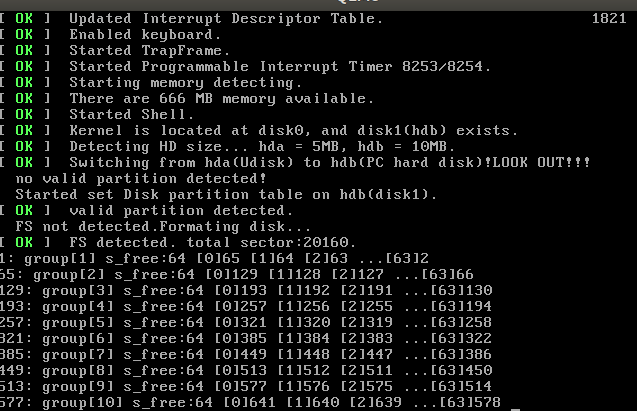
\includegraphics[width=14cm]{pic/assets/grouping_1}
        \caption{grouping(1)}	\label{grouping_1}	\end{figure}
        
末尾的几组如图~\ref{grouping_2}~所示.	

\begin{figure}[!htbp]
		\centering	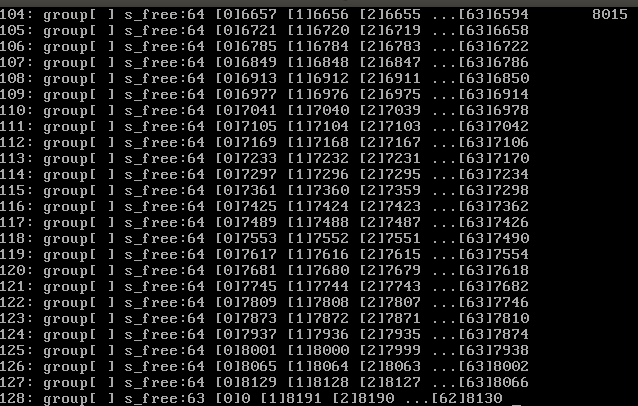
\includegraphics[width=14cm]{pic/assets/grouping_2}
		\caption{grouping(2)}	\label{grouping_2}	\end{figure}

注意,最后一组空闲块要少一个,而且最后一组没有下一组,s\_free\_blk\_nr[0] = 0;即下一组不存在.

第一次进入rios系统时,系统探测到磁盘上超级块的固定区域没有magic number判断出rifs尚未被建立,
故格式化硬盘,建立硬盘分区表,建立根目录.调用read和write将文件内容写入txt文件并读出到屏幕上显示.

第一次如图~\ref{first_rios}~所示.	

\begin{figure}[!htbp]
		\centering	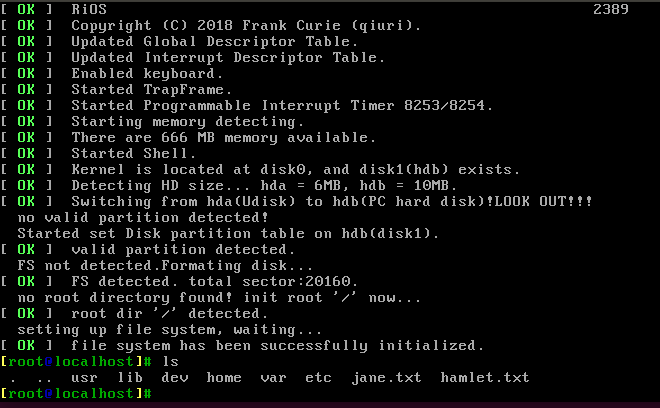
\includegraphics[width=14cm]{pic/assets/first_rios}
		\caption{第一次进系统}	\label{first_rios}	\end{figure}

下次进系统如图~\ref{next_rios}~所示.第二次(或以后)进入系统时,已经检测到magic number的存在,
故不再格式化磁盘,调用ls命令可见当前根目录下系统已经在上一次建立好了一些默认的文件夹,
而且并不会随着关机再开机而丢失,系统中我已经编写了键盘驱动和屏幕字符显示驱动,随着键盘敲击,
命令送入缓冲区,敲击回车时,命令送入命令解释程序即shell中解释运行,系统中先后调用
ls,cd qiuri,cd ..,pwd,mkdir dir1/dir2/dir3,cd dir1/dir2/dir3等,
可以看到测试效果良好,没有问题.	

\begin{figure}[!htbp]
		\centering	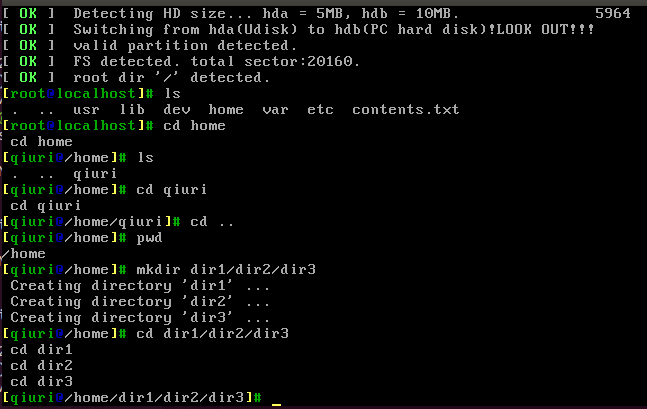
\includegraphics[width=14cm]{pic/assets/next_rios}
		\caption{下次进系统}	\label{next_rios}	\end{figure}


\subsection{空闲磁盘块的成组链接分配与回收方法}

成组链接方法是应该能够将之前的专用块(若闲置)给分配出去的,
上图是我不断申请新块,并将块号打印出来的情况,
可见我在分配了64号即第一组除了下一组之外的最后一个空闲块之后,开始转入第二组,
并从第二组中分配空闲块,然后下一次分配就能把之前的专用块(现已闲置)给分配出去,
即把1号分配出去了.如此下去,将如抽丝一般把整个磁盘上的磁盘块(包括不用的前专用块)给分配出去,

因为在做文件系统之前,我已经实现了设备管理,编写了IDE硬盘的驱动,
因而可以读写任意扇区,这里封装了hexdump 命令,可以把磁盘上任意一个扇区内容以十六进制打印出来,
从info disk命令中我们知道数据区从第521扇区开始,因为我们采取成组链接,
也按一定规律初始化了,故数据区第一个扇区的是存成组链接信息的.
在RiOS中数据区一个块两个扇区,故第一个有效的空闲区是第523扇区.该扇区用作某目录的数据区,图可见之前的.


\subsection{初始化}

为了基于空闲磁盘空间的成组链接方式的初始化,系统中有一个自定义的磁盘块联合体free\_space\_grouping\_head:

\begin{minted}{c}
union free_space_grouping_head {/*成组链接法,各组空闲块的头*/
	u16 bytes[512] = {0};/*占坑位 2 sectors*/
	struct {
		u16 s_free;
		u16 s_free_blk_nr[BLKS_PER_GROUP];/*[64]*/
	};
/*s_free_blk_nr[0] is next free group's nr*/
};	
\end{minted}

在rifs中,对于数据区,空闲磁盘空间管理采用成组链接方式,一个磁盘数据块有两个扇区,
这里采用了联合体而不是结构体,意义主要在于占位,使得一个这样的联合体恰好1024B即
两个扇区即一个数据块的大小,若此磁盘块为组里第一块,则它要记录整个组空闲块的信息,
第一项s\_free记录本组共有几个空闲块,其后的表项记录本组所有空闲块的块号,
其中s\_free\_blk\_nr[0]记录下一组的组号,若已经是最后一组,则s\_free\_blk\_nr[0]=0,
每次分配时s\_free-=1,然后以s\_free为数组下标,找到s\_free\_blk\_nr[]相应的空闲块号,
即为要分配的块号.若s\_free-=1后为0时,找下一组调入专用块,到下一组去找空闲块.


\section{目录项的确定}
如何得知一个目录文件里有多少个目录项?目录文件的inode中记录有大小i\_size,
由目录文件的inode中的i\_size得到目录文件大小.而struct dir\_entry目录项的大小是固定的,
由i\_size除以 sizeof(dir\_entry)可知有几个目录项目.

\section{多级索引}

教科书上Linux ext2多级索引原理示意图如图~\ref{Linux ext2 fs}~
\begin{figure}[!htbp]
	\centering	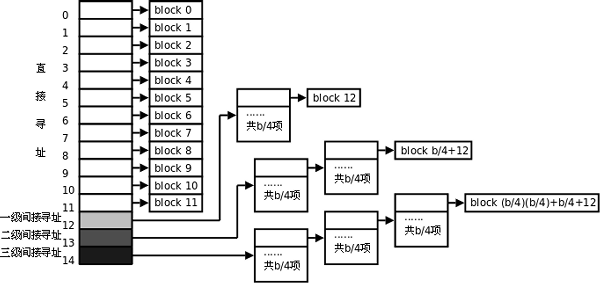
\includegraphics[width=14cm]{pic/assets/Linux_ext2_fs}
	\caption{Linux ext2}	\label{Linux ext2 fs}	\end{figure}

RiOS中的设定:

\begin{enumerate}
\item  zone[0~6]:	direct block 
\item  zone[7]:	    single indirect block
\item  zone[8]:	    double indirect block 
\item  zone[9]:	    trible indirect block
\end{enumerate}

大致估计一下容量.

\paragraph{直接寻址} zone[0~6]直接寻址: 

    每个块2扇区,7*(2*512)=7168B = 7kB

 length: 0~7(2512)B              [0,7168] B

 sector:length/512 	[1,7*2]

\paragraph{一次寻址} zone[7] 一次间址: 

    u16 zone[] u16 => 2B , 一个区可以存(2*512)/2=512 个扇区号,
    512 * (512*2) = 512kB.

 length: 7(2512)+1 ~ 7(2512)+512(5122) 

        [7169,531456]  B

 sector:$\left\lceil{length/512}\right\rceil$   $\sim$   [72+1,72+512*2]

[15,1038]      

\paragraph{两次寻址} zone[8] 两次间址: 512 * 512 * (512 * 2)= 256 MB 

 length:  7(2*512)+512(512*2)+1 $\sim$ 7(2512)+512(5122)+512512(512*2)

 	[531457,268966912] B

 sector:$\left\lceil{length/512}\right\rceil$  $\sim$    [72+5122+1,?]	

 	[1039,525326]

\paragraph{三次寻址} zone[9] 三次间址: 512 * 512 * 512 * (512 * 2) = 128 GB 

 length: 7*(2*512)+512 * (512 * 2)+512 * 512 * (512*2)+1 $\sim$  7*(2*512)+512(512*2)+512*512(512*2)+512 * 512 * 512 * (512 * 2)

[268966913,137707920384] B

三次间址理论上支持很大容量,但实际上做实验用不到那么多.

\subsection{删除文件}

删除文件相对来说比较麻烦,但不是很困难,但要仔细.分几种情况讨论,从直接寻址到一次寻址,
再到两次寻址,犹如一个分段函数.

\begin{minted}{c}   
void rm(const char *name,u8 mode)
{
	int fd = open(name);if(fd==-1)return;
	int contents_len = current->filp[fd]->f_inode->i_size;
	if( current->filp[fd]->f_inode->i_size==0){
		kprintf("\n rm: '%s': not a valid file.",name);
		return;
	}
	if(current->filp[fd]->f_inode->i_nlinks!=0)
		kprintf("\n rm: nlinks:%d",current->filp[fd]->f_inode->i_nlinks);
	u16 ino = current->filp[fd]->f_inode->i_ino;
	int length = current->filp[fd]->f_inode->i_size;
	close(fd);
	if(ino==0) _panic(" FBI WARNING:rm:i_ino = 0 !!! ");/* will destroy root directory */
/* free blocks and then free inode,finally remove this record from the directory */	
	u8 sector[512]={0};int buffer_offset=0;
	int total_sectors = (length+511)/512;
	struct m_inode rm_inode;
	iget(&rm_inode,ino);

	memset(sector,0x00,sizeof(sector));
	if(total_sectors<=7*SECTOR_PER_BLOCK){
/* @#0.1 zone[0~6]: direct block 直接寻址,大概7kB*/
		for(int i=0; i<total_sectors; i++){
			int blk_i = get_zone_blks(i+1)-1;
			if(i%2==0){
				IDE_write_sector((void *)&sector, DATA_BLK_NR_TO_SECTOR_NR(rm_inode.i_zone[blk_i]));
			}else{
				IDE_write_sector((void *)&sector, DATA_BLK_NR_TO_SECTOR_NR(rm_inode.i_zone[blk_i])+1);
				if(rm_inode.i_zone[blk_i]!=0)free_block(rm_inode.i_zone[blk_i]);	
			}
		}
	}else if(total_sectors<=7*SECTOR_PER_BLOCK+512*SECTOR_PER_BLOCK){
/* @#1.1 zone[0~6]: direct block 直接寻址,大概7kB*/		
		for(int i=0; i<7*SECTOR_PER_BLOCK; i++){
			int blk_i = get_zone_blks(i+1)-1;
			if(i%2==0){
				IDE_write_sector((void *)&sector, DATA_BLK_NR_TO_SECTOR_NR(rm_inode.i_zone[blk_i]));
			}else{
				IDE_write_sector((void *)&sector, DATA_BLK_NR_TO_SECTOR_NR(rm_inode.i_zone[blk_i])+1);	
				if(rm_inode.i_zone[blk_i]!=0)free_block(rm_inode.i_zone[blk_i]);
			}
		}
/*  #1.2 zone[7]:   single indirect block 一次间址,大概五百kB*/
		u8 two_sectors[1024]={0};/*load indexs in zone[7] to memory 'two_sectors'*/
		IDE_read_sector((void *)two_sectors, DATA_BLK_NR_TO_SECTOR_NR(rm_inode.i_zone[7]));
		IDE_read_sector((void *)(two_sectors + 512), DATA_BLK_NR_TO_SECTOR_NR(rm_inode.i_zone[7])+1);
		u16 * pzone =(u16 *)&two_sectors;/* that's right */

		for(int i = 7*SECTOR_PER_BLOCK;i<total_sectors;i++){//[7*2+1,7*2+512*2]
			int blk_i = get_zone_blks(i+1)-1;
			u16 zone_index = pzone[blk_i-7];/*zone[0~6]*/
/* MAKE SURE that zone_index!=0. assert(zone_index!=0)*/			
			if(zone_index==0) {
				_panic("FBI WARNNING:rm:zone_index should not be zero!!!");/* will destory root directory!*/			
			}
			if(i%2==0){
					IDE_write_sector((void *)&sector, DATA_BLK_NR_TO_SECTOR_NR(zone_index));
			}else{
					IDE_write_sector((void *)&sector, DATA_BLK_NR_TO_SECTOR_NR(zone_index)+1);
					if(zone_index!=0)free_block(zone_index);
			}
		}

		if(rm_inode.i_zone[7]!=0)free_inode(rm_inode.i_zone[7]);
	}
	else if(total_sectors<=7*SECTOR_PER_BLOCK+512*SECTOR_PER_BLOCK+512*512*SECTOR_PER_BLOCK){
/* @#2.1 zone[0~6]:  direct block 直接寻址,大概7kB*/	
		kprintf("\n  rm: removing direct blocks of file '%s'.",name);
		for(int i=0; i<7*SECTOR_PER_BLOCK; i++){
				int blk_i = get_zone_blks(i+1)-1;
				if(i%2==0){
					IDE_write_sector((void *)&sector, DATA_BLK_NR_TO_SECTOR_NR(rm_inode.i_zone[blk_i]));
				}else{
					IDE_write_sector((void *)&sector, DATA_BLK_NR_TO_SECTOR_NR(rm_inode.i_zone[blk_i])+1);	
					if(rm_inode.i_zone[blk_i]!=0)free_block(rm_inode.i_zone[blk_i]);
				}
		}
/*  #2.2 zone[7]  :  single indirect block 一次间址,大概五百kB*/
		kprintf("\n  rm: removing single indirect blocks of file '%s'.",name);
		u8 two_sectors[1024]={0};/*load indexs in zone[7] to memory 'two_sectors'*/
		IDE_read_sector((void *)two_sectors, DATA_BLK_NR_TO_SECTOR_NR(rm_inode.i_zone[7]));
		IDE_read_sector((void *)(two_sectors + 512), DATA_BLK_NR_TO_SECTOR_NR(rm_inode.i_zone[7])+1);
		u16 * pzone =(u16 *)&two_sectors;/* that's right */

		for(int i = 7*SECTOR_PER_BLOCK;i<7*SECTOR_PER_BLOCK+512*SECTOR_PER_BLOCK;i++){//[7*2+1,7*2+512*2]
			int blk_i = get_zone_blks(i+1)-1;
			u16 zone_index = pzone[blk_i-7];/*zone[0~6]*/
/* MAKE SURE that zone_index!=0. assert(zone_index!=0)*/			
			if(zone_index==0) {
				_panic("FBI WARNING:read:zone_index should not be zero!!!");/* will destory root directory!*/			
			}
			if(i%2==0){
					IDE_write_sector((void *)&sector, DATA_BLK_NR_TO_SECTOR_NR(zone_index));
			}else{
					IDE_write_sector((void *)&sector, DATA_BLK_NR_TO_SECTOR_NR(zone_index)+1);
					if(zone_index!=0)free_block(zone_index);
			}
		}
		for(int i=0;i<512;i++){
			if(pzone[i]!=0)
				free_block(pzone[i]);
		}
		if(rm_inode.i_zone[7]!=0)free_inode(rm_inode.i_zone[7]);
/*  #2.3 zone[8]  :  double indirect block 两次间址,支持大概256MB*/
		kprintf("\n  rm: removing double indirect blocks of file '%s'.",name);
		memset(two_sectors,0x00,sizeof(two_sectors));/*reuse that buffer*/
		memset(sector,0x00,sizeof(sector));
		if(rm_inode.i_zone[8]==0){/* allocate newblock for  zone[8] */
			_panic("FBI WARNING:rm:file's i_zone[8] is NOT allocated!!!"); 
		}
		/*load indexes in zone[8] to memory 'two_sectors'*/
		IDE_read_sector((void *)two_sectors, DATA_BLK_NR_TO_SECTOR_NR(rm_inode.i_zone[8]));
		IDE_read_sector((void *)(two_sectors+512), DATA_BLK_NR_TO_SECTOR_NR(rm_inode.i_zone[8])+1);
		u16 * p_zone = (u16 *)&two_sectors;
		u8 double_sectors[1024]={0};/* double indirect block buffer*/
		u16 * pd = (u16 *)&double_sectors;
		for(int i=7*SECTOR_PER_BLOCK+512*SECTOR_PER_BLOCK;i<total_sectors;i++){
			/* load single indirect block (zone[8]) to memory, two_sectolrs <= zone[8]  */			
			IDE_read_sector((void *)two_sectors, DATA_BLK_NR_TO_SECTOR_NR(rm_inode.i_zone[8]));
			IDE_read_sector((void *)(two_sectors+512), DATA_BLK_NR_TO_SECTOR_NR(rm_inode.i_zone[8])+1);
			int blk_i = get_zone_blks(i+1)-1;
			u16 single_indirect_i =(blk_i-7-512)/512;/*zone[0~6]:7 zone[7]:512*/
			u16 double_indirect_i = (blk_i-7-512) -512*single_indirect_i;

			u16 si_zone_index = p_zone[single_indirect_i];
			if(si_zone_index ==0) _panic("FBI WARNING:read:file's si_zone_index has not been allocated!!!");
			/* get double indirect block from disk */
			IDE_read_sector((void *)double_sectors, DATA_BLK_NR_TO_SECTOR_NR(si_zone_index));
			IDE_read_sector((void *)(double_sectors+512), DATA_BLK_NR_TO_SECTOR_NR(si_zone_index)+1);
			/* ok, double indirect block is now loaded to double_sectors in memory */	
			u16 db_zone_index = pd[double_indirect_i];
  			if(db_zone_index==0) _panic("FBI WARNING:read:file's db_zone_index has not been allocated!!!");
			/*load file contents been from disk*/
			if(i%2==0){
				 IDE_read_sector((void *)&sector , DATA_BLK_NR_TO_SECTOR_NR(db_zone_index));
			}else{
				 IDE_read_sector((void *)&sector , DATA_BLK_NR_TO_SECTOR_NR(db_zone_index)+1);
				 if(db_zone_index!=0)free_block(db_zone_index);
			}
		}
		for(int i=0;i<512;i++){
			if(p_zone[i]!=0)
				free_block(p_zone[i]);
		}
		if(rm_inode.i_zone[8]!=0)free_inode(rm_inode.i_zone[8]);
	}
	else{
		kprintf("\n file size: %d Bytes.",length);
		_panic(" FBI_WARNING:rm:your file is TOO LARGE!!!");
	}

/* ok, after we have freed its data blocks, we can free its inode*/
	memset(&rm_inode,0x00,sizeof(rm_inode));
	iput(&rm_inode,ino);
	free_inode(ino); 
/* remove its infomation from the directory */
	memset(sector,0x00,sizeof(sector));
	struct dir_entry *de = (struct dir_entry *)NULL;
/*it will rm file under current directory.   */
	IDE_read_sector((void *)&sector, DATA_BLK_NR_TO_SECTOR_NR(current->pwd->i_zone[0]));	
	de = (struct dir_entry*)sector; 
	/* in case that two directory have the same name */
	if(get_dir((char *)name)==-1){
		kprintf("\n WARNING:rm:the file '%s' does NOT exist.",name);
		return ;
	}
/*we should control the length of file name,otherwise may run into problem*/
	if( strlen(name) > MAX_NAME_LEN) 
		_panic("FBI WARNING:length of dir name must under 14 chars!\n halt...");//MAX_NAME_LEN		
	int i=0;
	for(i=0;i<current->pwd->i_size/sizeof(struct dir_entry);i++){
		if(equal_to((char *)de->name,name)) break ;
		de++;
	}	/*point to correct position*/
	memset(de,0x00,sizeof(struct dir_entry));
	struct dir_entry *de2 = (struct dir_entry *)NULL;
	if(i==current->pwd->i_size/sizeof(struct dir_entry)){
/* if it is the last one */		
		goto writeback;
	}
	de2=de; de2++;
	for(int j=0;j<current->pwd->i_size/sizeof(struct dir_entry)-i;j++){
		* de = * de2;
		de++;de2++;
	}
writeback:
	IDE_write_sector((void *)&sector, DATA_BLK_NR_TO_SECTOR_NR(current->pwd->i_zone[0]));	
/*ok, update current directory file's filesize, because we removed a record.*/	
	current->pwd->i_size -= 1 * sizeof(struct dir_entry);	/* remove a dir*/
	iput(current->pwd,current->pwd->i_ino);
	kprintf("\n  rm: file '%s' has been successfully removed.",name);
	return;
}

\end{minted}





% \clearpage 

\chapter{运行与测试} 
%\pagenumbering{arabic} % 阿拉伯数字页码
本工程的性质是简易操作系统内核(当然还不算很完整),与Windows
下的exe文件性质不同,因此有必要谈谈如何运行测试.这里谈两种,
一是在物理裸机上运行,二是利用虚拟机完成运行测试;从学习原理的目的
出发,折腾前一种没有多大必要,而且可能有格式化硬盘的危险,还是推荐后一种方法.

\section{物理裸机}
\subsection{GRUB}
安装GRUB2到U盘的方法已经讲过,这里主要就是把编译后生成的build目录下的grub.cfg
和kernel.bin拷贝到U盘的相应位置即可.可能没有权限,用sudo cp的办法可以实现.
这里一定要注意路径的问题,路径放得不对就没有效果了.

如图~\ref{grub_folder01}~及图~\ref{grub_folder02}~所示.		

\begin{figure}[!htbp]
		\centering	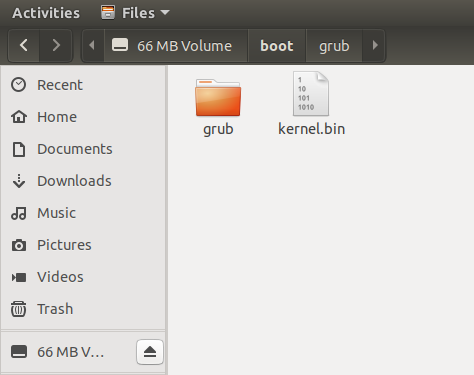
\includegraphics[width=14cm]{pic/assets/testcase/grub_folder01}
		\caption{U盘目录01}	\label{grub_folder01}	\end{figure}



\begin{figure}[!htbp]
		\centering	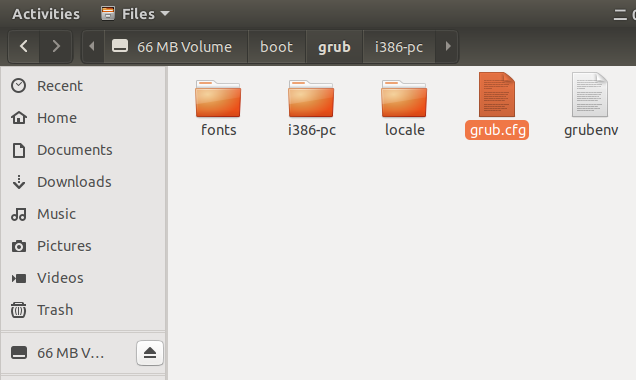
\includegraphics[width=14cm]{pic/assets/testcase/grub_folder02}
		\caption{U盘目录02}	\label{grub_folder02}	\end{figure}

U盘拷贝完的结构如图~\ref{grub_folder01}~所示.

\begin{figure}[!htbp]
		\centering	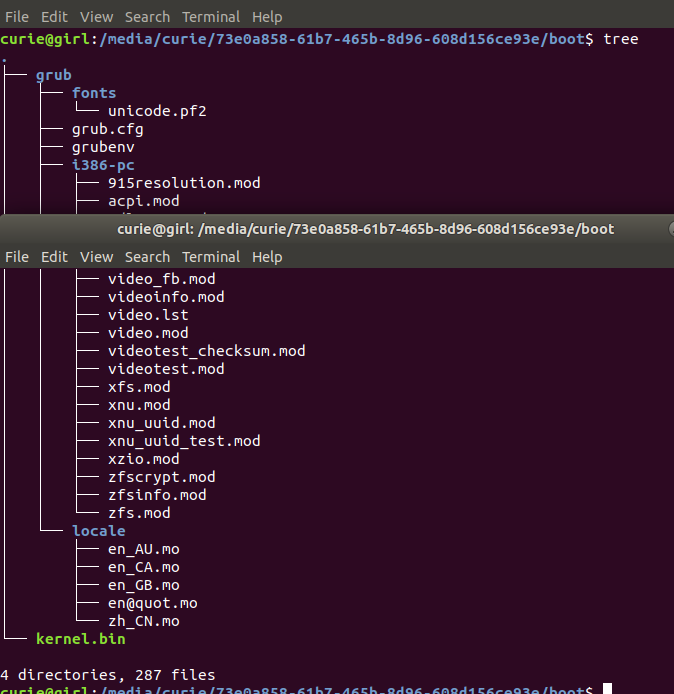
\includegraphics[width=14cm]{pic/assets/testcase/grub_tree}
        \caption{U盘目录02}	\label{grub_tree}	\end{figure}
        
好,接下来和U盘装系统的步骤应该差不多了,不过值得注意的是,为了建立文件系统,第一次进系统时,
我将把格式化整个物理硬盘,要注意数据的备份,比较危险.因为这个原因,在内核写到文件系统之前,
均在裸机上进行过验证性测试,之后因为要格式化硬盘的原因,只在qemu上测试了.把生成的
RiOS-i386.iso镜像通过其他途径烧写到U盘应当可行,不过没有在物理机器上验证过需要格式化,有一定风险,
请慎重!
早期系统测试结果如图~\ref{machine}~所示.

\begin{figure}[!htbp]
    \centering	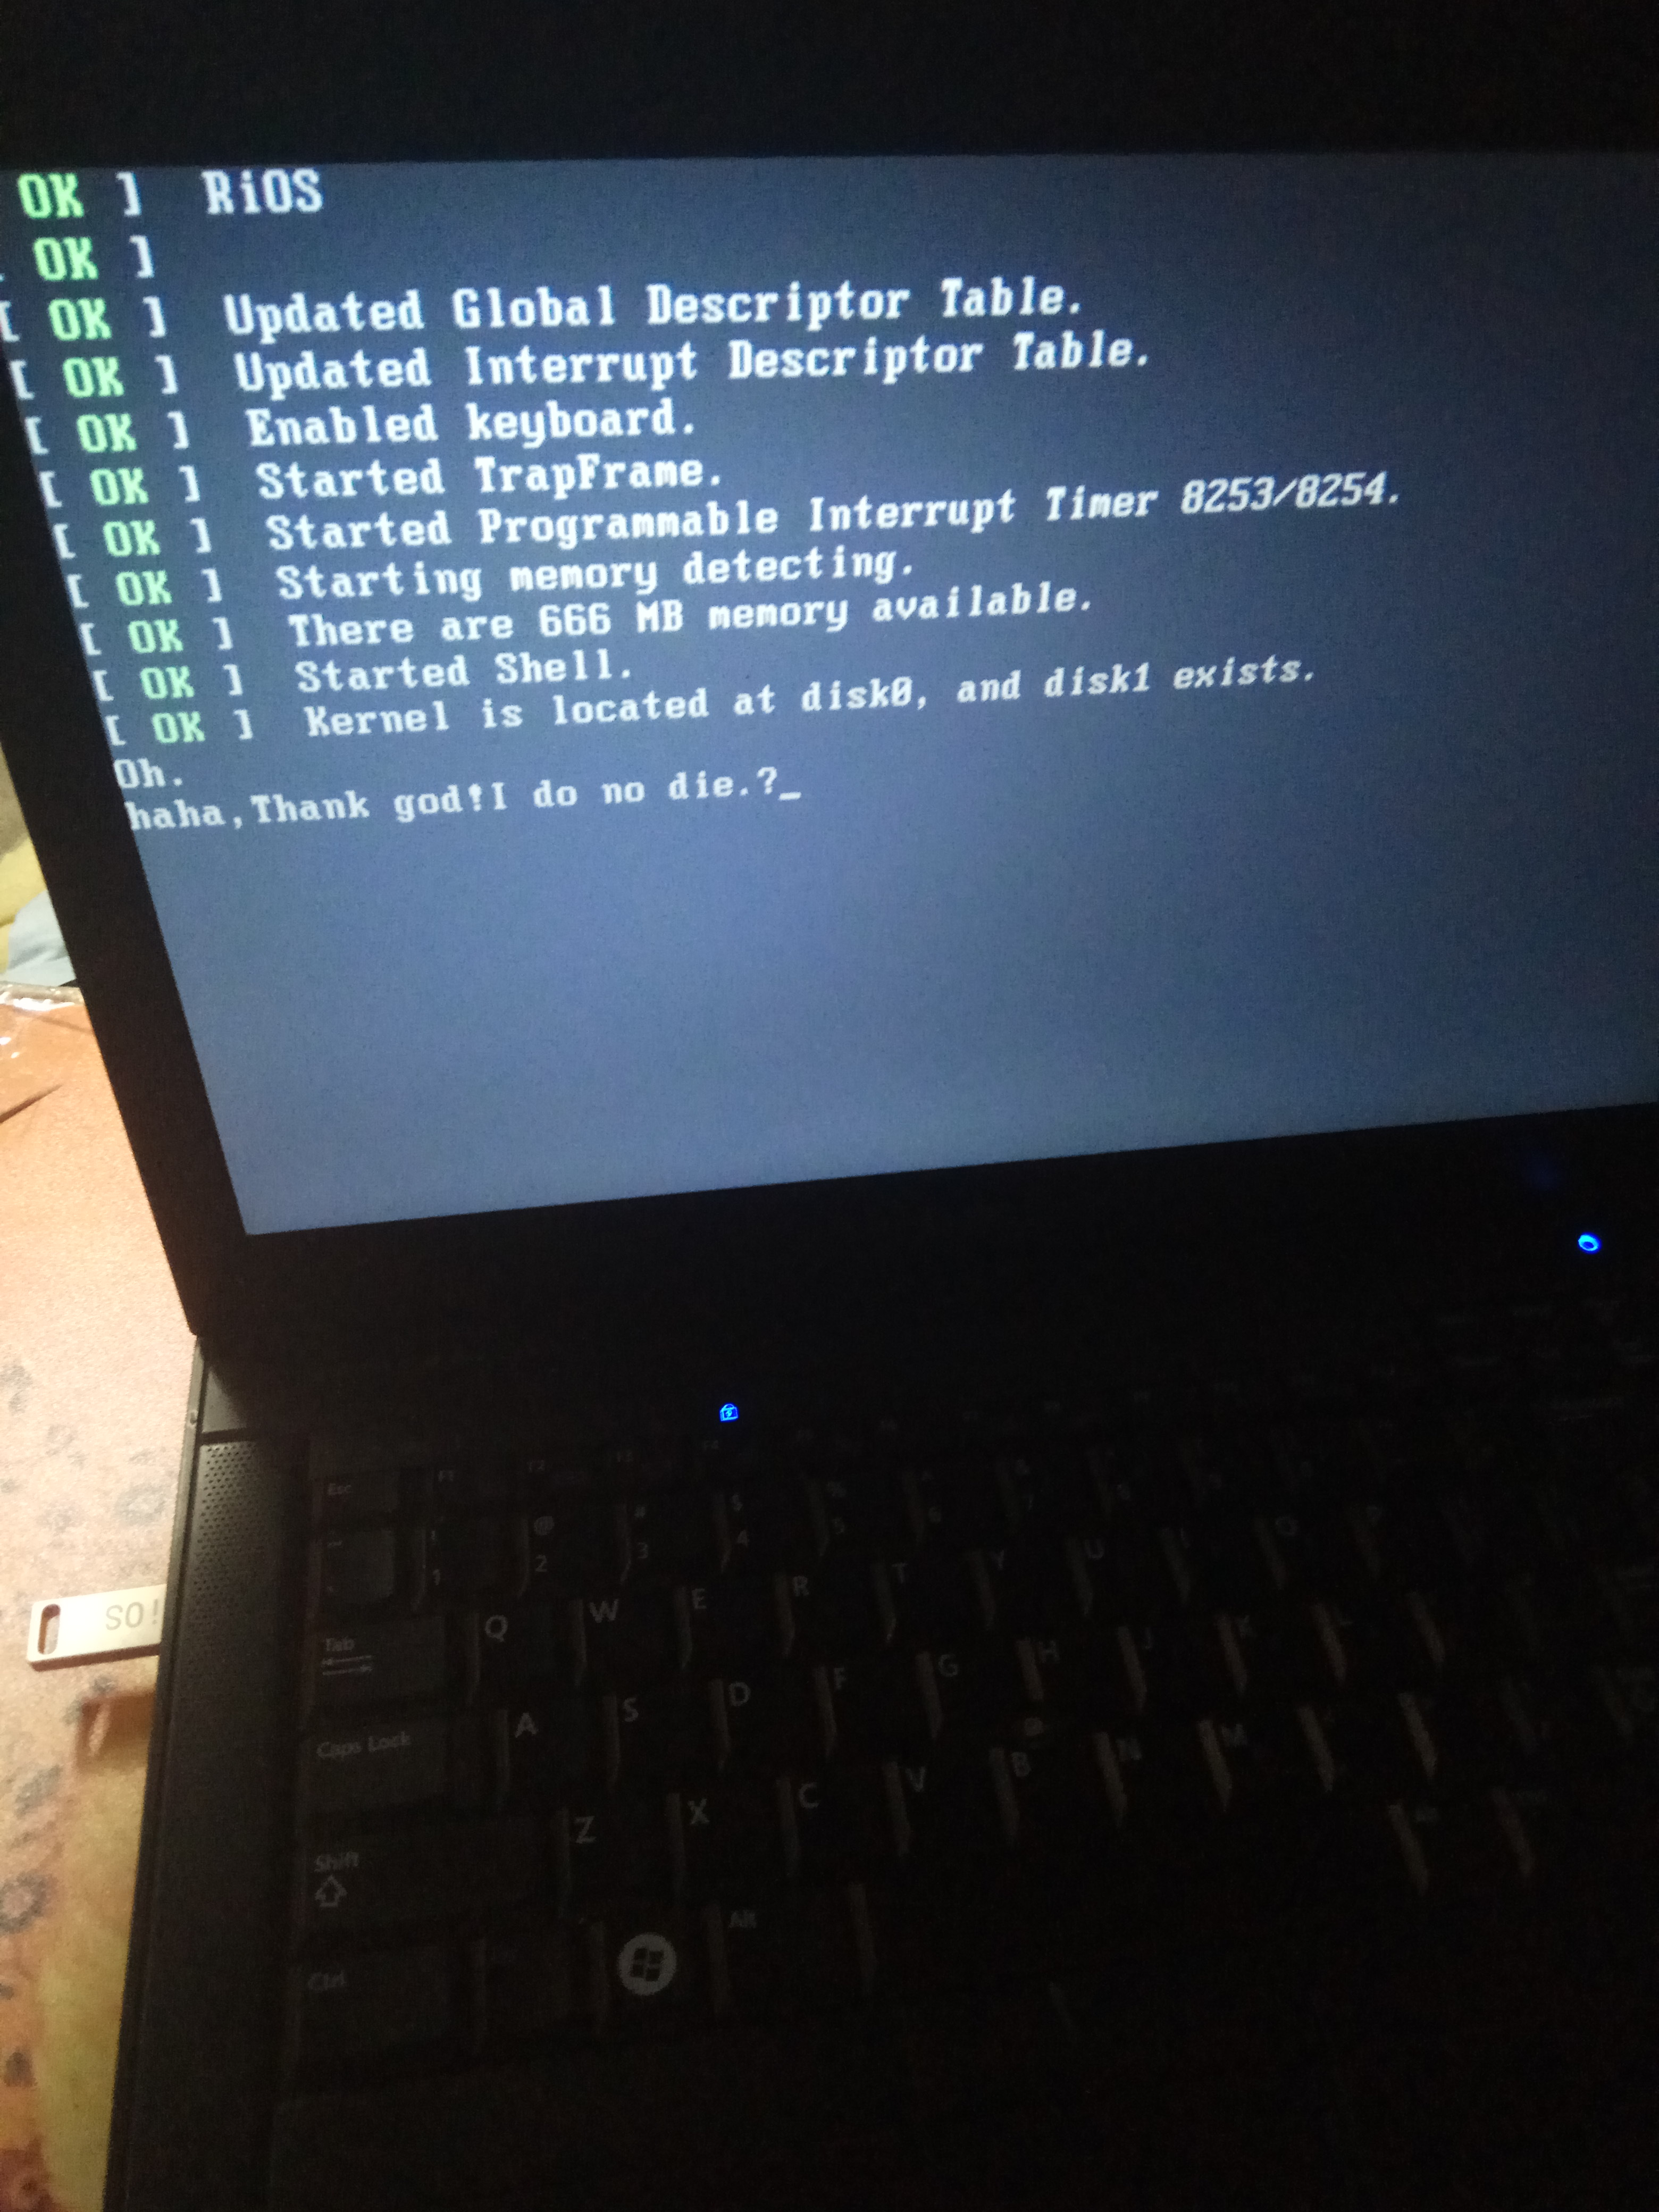
\includegraphics[width=10cm]{pic/assets/testcase/machine}
    \caption{早期裸机测试(非目前最终版本)}	\label{machine}	\end{figure}

\section{利用QEMU模拟器测试}

这里我们开发所用的宿主机操作系统为Ubuntu,笔者用的是Ubuntu17.04,(后来升级到18.04).
请先安装好依赖.
\begin{minted}{shell}
# 之前应该已安装grub2
sudo apt-get install gcc
sudo apt-get install xorriso
# 安装xorriso 才能执行grub-mkrescue
sudo apt-get install qemu
\end{minted}

目前我的机器环境已经配置好,以上是大致回忆的要安装的东西,可能不完整.若还有依赖,请自行安装和配置.
接下来可以进入我的代码文件夹,也可以从github网站上下载.

\begin{minted}{shell}
git clone https://github.com/Twopothead/baby-rios
cd baby-rios
make
\end{minted}

系统测试结果如图~\ref{r1}~所示.

\begin{figure}[!htbp]
    \centering	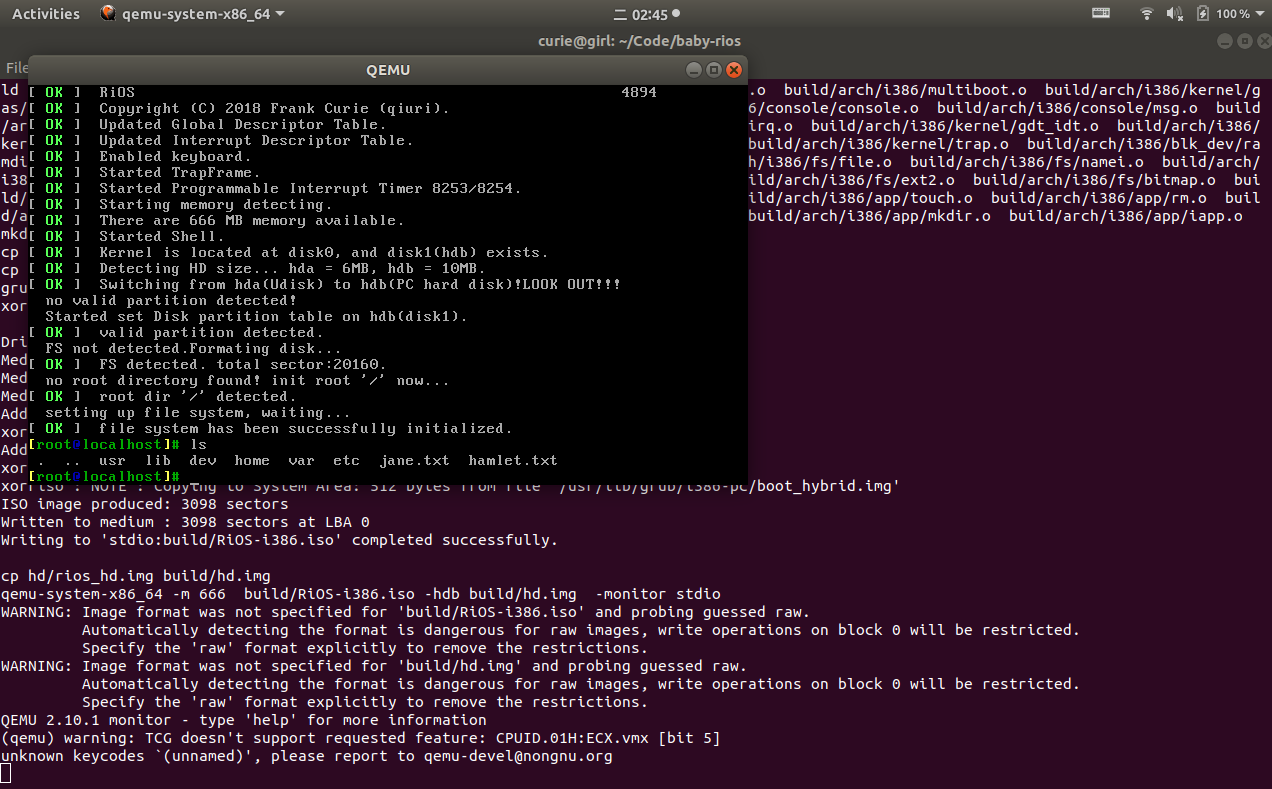
\includegraphics[width=14cm]{pic/assets/testcase/r1}
    \caption{第一次进系统}	\label{r1}	\end{figure}

\begin{minted}{shell}
#这里的命令不是在Ubuntu中运行,而是在qemu虚拟机中使用
ls
cd home
cd qiuri
cd /
cd var
ls 
cd /
cd etc
ls
cd getty
ls
cd /
mkdir dir1/dir2/dir3
ls
cd dir1/dir2/dir3
ls
cd ..
ls
clear
cd /
help
pwd
cd home/qiuri
pwd
info superblock
info disk
info grouping
ls
cd ..
ls
rmdir qiuri
ls
cd ..
ls
rmdir home
ls
cat hamlet.txt
cat jane.txt
ls
rm hamlet.txt
\end{minted}

当然cat jane.txt可能显示过快,看不清楚,系统中还可以使用slowcat jane.txt来显示,
这样可以看清楚了,不过要把一本书从头到尾打印到屏幕,前者要1分钟,后者可能要一下午了.

系统测试结果2如图~\ref{r2}~所示.

\begin{figure}[!htbp]
    \centering	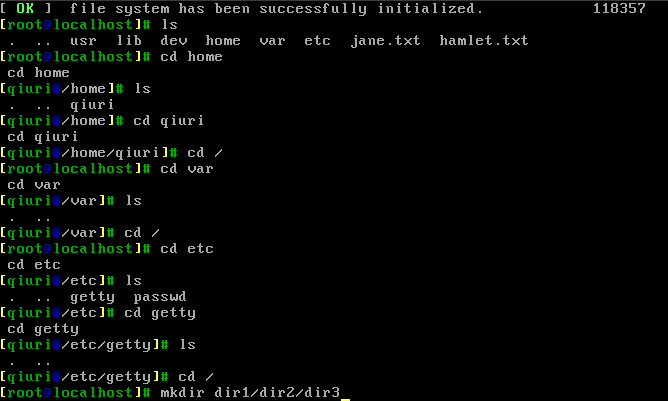
\includegraphics[width=14cm]{pic/assets/testcase/r2}
    \caption{系统测试2}	\label{r2}	\end{figure}

系统测试结果3如图~\ref{r3}~所示.

\begin{figure}[!htbp]
    \centering	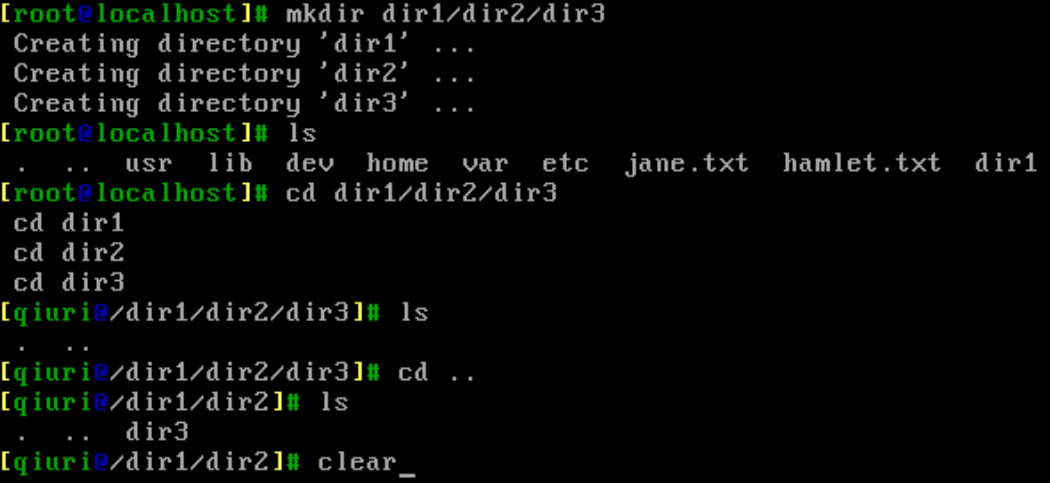
\includegraphics[width=14cm]{pic/assets/testcase/r3}
    \caption{系统测试3}	\label{r3}	\end{figure}

系统测试结果4如图~\ref{r4}~所示.

\begin{figure}[!htbp]
    \centering	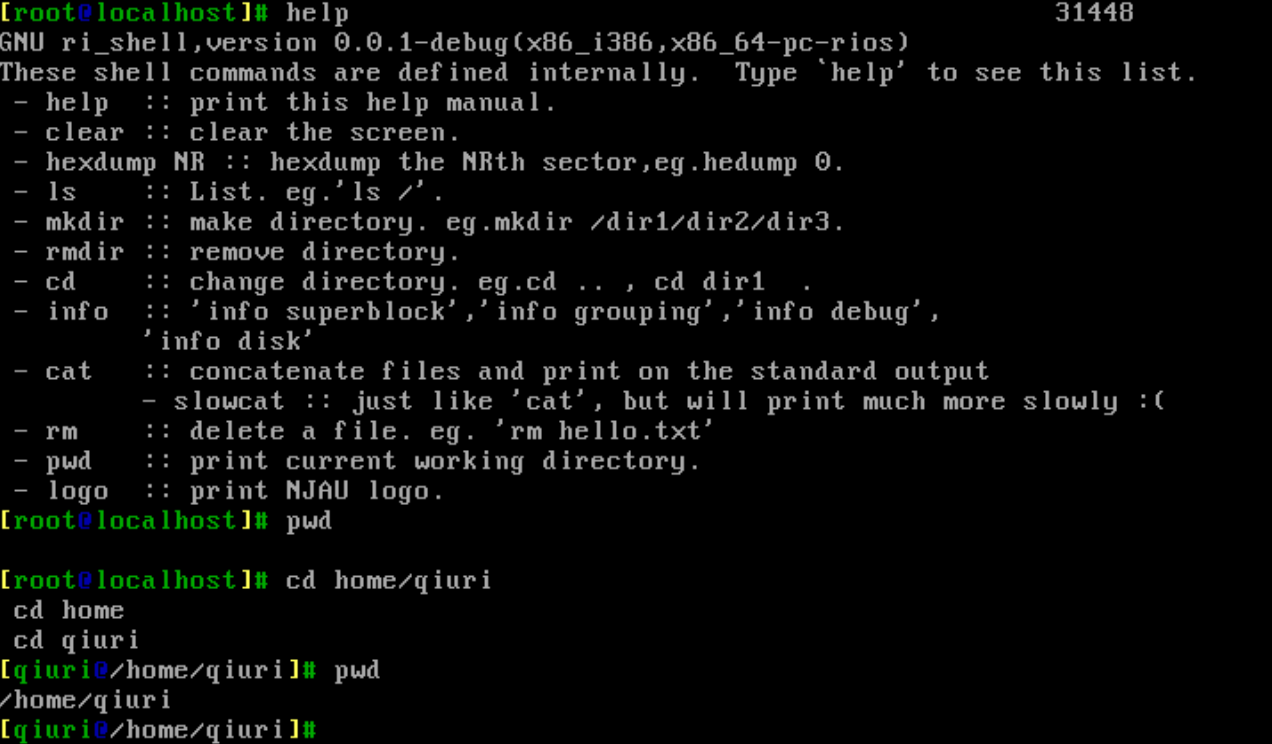
\includegraphics[width=14cm]{pic/assets/testcase/r4}
    \caption{系统测试4}	\label{r4}	\end{figure}

系统测试结果5如图~\ref{r5}~所示.

\begin{figure}[!htbp]
    \centering	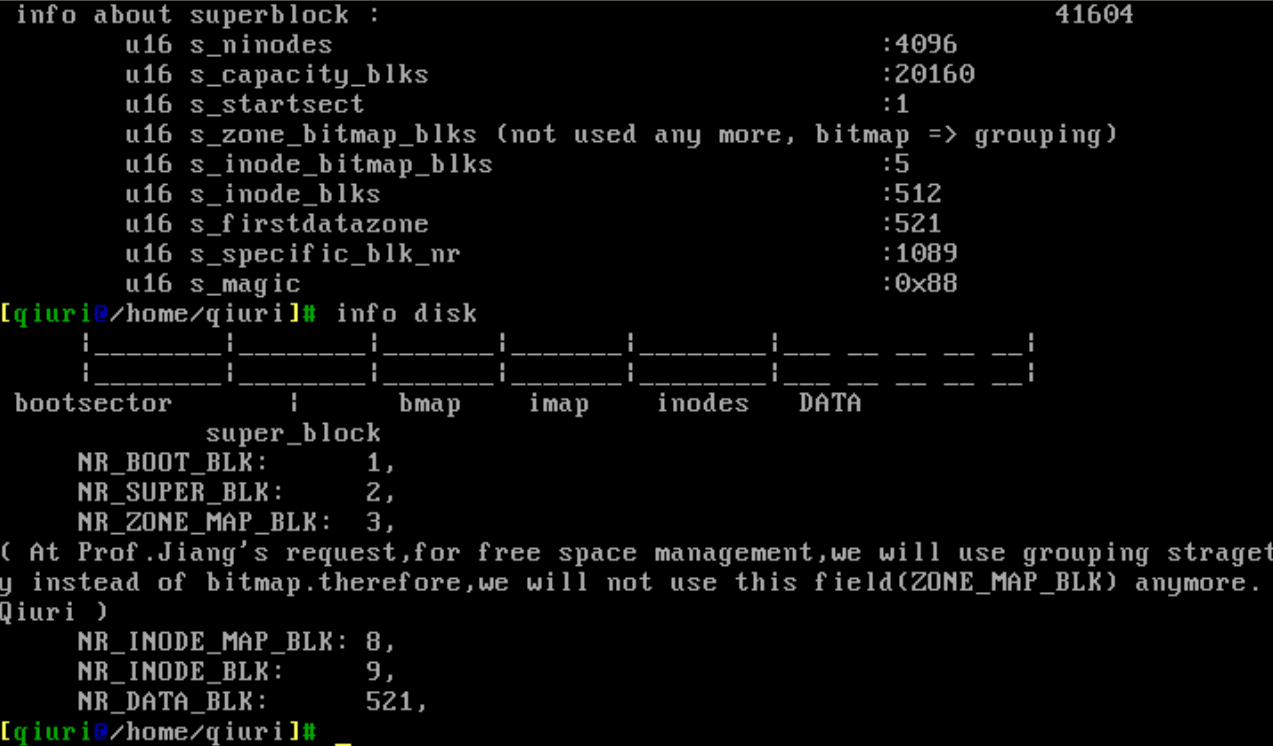
\includegraphics[width=14cm]{pic/assets/testcase/r5}
    \caption{系统测试5}	\label{r5}	\end{figure} 

系统测试结果6如图~\ref{r6}~所示.

\begin{figure}[!htbp]
    \centering	\includegraphics[width=14cm]{pic/assets/testcase/r6}
    \caption{系统测试6}	\label{r6}	\end{figure} 

系统测试结果7如图~\ref{r7}~所示.

\begin{figure}[!htbp]
    \centering	\includegraphics[width=14cm]{pic/assets/testcase/r7}
    \caption{系统测试7}	\label{r7}	\end{figure} 

系统测试结果8如图~\ref{r8}~所示.

\begin{figure}[!htbp]
    \centering	\includegraphics[width=14cm]{pic/assets/testcase/r8}
    \caption{系统测试8}	\label{r8}	\end{figure}    

以上为第一次进系统,我们可以把qemu关掉,再在Ubuntu终端使用make qemu或make run命令
再次进系统.初始化时,系统中有jane,txt(大文件)和hamlet.txt(小文件).
当我们再次进系统时可以看到,因为上次关机时删去了hamlet.txt,故系统中只剩jane.txt.
若上次开机时建立了新目录且没被删掉的话,则下次开机仍能够看到
\begin{minted}{shell}
#这里的命令不是在Ubuntu中运行,而是在qemu虚拟机中使用
ls
cat jane.txt
ls
mkdir dir1/dir2/dir3
\end{minted}

以后要再次进系统可以在Ubuntu终端使用make qemu或make run命令.

如图~\ref{s1}~所示.

\begin{figure}[!htbp]
    \centering	\includegraphics[width=14cm]{pic/assets/testcase/s1}
    \caption{再次进系统测试1}	\label{s1}	\end{figure}  

如果要重新编译,重新建立文件系统.应使用make clean,然后再make.可以自行测试.
    
% \begin{minted}{c}
%     int main() {
%         printf("hello, world");
%         return 0;
%     }
% \end{minted}



% \clearpage 

\chapter{总结与展望} 
% \pagenumbering{arabic} % 阿拉伯数字页码

\section{致谢}
感谢姜老师的耐心指导和方向上的提醒,我的问题是理论知识不扎实就动手干,
这样的后果常常是陷入迷茫,没有方向,常常纠结下一步要写什么代码,这是理论知识欠缺的表现.

最初打算写本项目是因为组队参加"龙芯杯"遭遇的彻底失败,这次失败使我意识到自己与他人的巨大差距,发现自己
学的课程没有联系起来,从而形成解决实际问题的综合能力,觉得需要做一个接近底层的综合性项目.感谢赵老师的
悉心指点与支持鼓励.

还要感谢朋友以及同学们项目中带给的大力支持和帮忙,给我带来极大的启发。
也要感谢参考文献中的作者们,通过他们的文章或著作,使我对项目有了很好的出发点。

\section{总结}

个人觉得本次课程设计难度比较大,对我是一次综合性考验.课设所用知识包括
操作系统原理、微机原理、汇编语言、数据结构、Linux命令等,还要涉及GAS汇编、Makefile编写、GRUB格式、
ATA硬盘串口驱动等零碎知识,这些做项目之前也都不懂,需要查阅很多资料.当程序出现奇怪的bug调不出来时,
一个人常常感到莫大的孤独.

文件管理虽然是相对独立的一章,但若要想在物理的机器上做出来,必须先写设备驱动,要键盘输入有反应,屏幕能够响应,
还得写中断处理程序和字符设备驱动,在此之前要先正确设置好gdt表和idt表,内存管理也需要能够malloc和free,
本系统还完成了简单的连续内存分配和对8259A,8253或其兼容芯片的编程.
所有这些必须正确做完才能进入文件系统的编写.怎样才能符合grub规范,
如何才能读写物理IDE硬盘扇区,如何写串口驱动.这些在我做此次课设之前,我也不清楚.
我阅读了文献和源代码之后,才有初步的认识,自己在编写代码和调试bug的过程中,
才逐步深入了解.当我遇到困难做不下去时,就多找几个这方面的材料对比着看.

当有人问Linus如何深入理解minix内核时,他提出"RTFSC":去读源码吧.这里RTFSC体现了阅读源码的艰辛和重要性.
.
在操作系统的学习中,我一直结合赵炯 那本书阅读Linux0.11源码,虽然艰难,但有时也会感到很有趣,
有时会发现比较实现起来很复杂的一件事,Linux代码几笔带过,实现得简洁有力,这是多么精妙!
Linux0.11是适合初学者的源码,同样的还有用于教育目的的经典的xv6内核,
国内有在jos和xv6基础上改的ucore实验,也可以看看.
我在课程设计进行中部分阅读了其他不知名的小kernel.真正仔细研究的是Linux0.11,xv6和ucore这三套源码,
阅读源码不会一帆风顺,当我遇到困难时,就把三个对比着看,看他们面对同样问题是如何处理的,从中收获很多.
Github和osdev网站也给我帮助.

网上关于简易内核编写的资料并不是很少,但关于文件系统的实现上,大多是实现已有文件系统
,最常见的是基于fat32,这其实是比较简单的,还有的是完全实现ext2甚至ext4文件系统,这个难度相当大,
我认为这不是普通学生能够在短时间做出来的.
实现一个自定义的文件系统难度应该在二者之间,也还是可以做到的,但在实践中越往后写下去越难找到可参考的资料,
水平有限,我也花费了很多时间.

在这一点上Linux0.11实现的是minix文件系统,xv6和ucore实现的是sfs文件系统,
由于minix文件系统和sfs都是已知的文件系统,这几个在交叉开发时可以采用mkfs命令做出一个磁盘镜像
,然后可以考虑和内核镜像做成系统集成盘.但这情况不适用于我们的RiOS,因为我的文件系统是自定义的,
除非自己写个类似mkfs的程序,否则想用mkfs命令做出相应磁盘镜像是不可能的.
最后,我采用系统探测磁盘并格式化的方法解决了这一问题.
至于空闲块成组链接,我也是反复研究课本,弄懂理论后摸索着写代码.

\subsection{存在问题}

"得失寸心知",为此项目颇费了一番精力,其中我也走过很多弯路,快乐与痛苦、优点与不足自己是最清楚的.
这里谈谈缺陷.本项目基本完整地实现了操作系统中文件系统部分,但是严格地说它并不能算得上一个整体结构完整的
简单内核.因为个人水平和时间精力有限,并没有实现进程管理,这是遗憾.内存管理使用了较为原始的方法,虽然
能够支持系统的运行,但不利于多进程的管理.

\subsection{展望}

不知道是否有同学对继续编写此项目有兴趣,如果真的有,那我将很高兴.
目前内核要做的工作很明显,一是把内存管理由最初的原始方法替换为段页式内存管理,
有了多进程在内存管理方面的基础,可以考虑实现真正的进程调度.后者如何实现,前面已经有相关论述,
应该说后者的基础工作(除了段页式内存管理),现在还是有的.若完成了这些,整个项目应该能够大体覆盖书上的
一些知识点了.还在网上看过\href{https://legacy.gitbook.com/book/nju-ics/ics2017-programming-assignment/details}{ics-pa实验},比较有趣
,我也挺想移植一个小游戏到我们的内核上去,不过限于水平和时间精力,没有付诸行动.
未来合适的时候,我可能还会在\href{https://github.com/Twopothead/baby-rios}{github}继续发展此项目,如果有想法,欢迎与我交流.






% \clearpage
\addcontentsline{toc}{chapter}{参考文献}
\zihao{5}

%% \bibliographystyle{gbt7714-2005}
%% \bibliography{my.bib}

%%完成后再改成thebib...
\begin{thebibliography}{99}
% \bibitem{ck1} Crosby M J, Karnopp D C. System for controlling the transmission of energy between spaced members: U.S. Patent 3,807,678[P]. 1974-4-30.
% \bibitem{ck2} Crosby M J, Karnopp D C. System for controlling the transmission of energy between spaced members: U.S. Patent 3,807,678[P]. 1974-4-30.
% \bibitem{ck3} Crosby M J, Karnopp D C. System for controlling the transmission of energy between spaced members: U.S. Patent 3,807,678[P]. 1974-4-30.
\bibitem{ck1}Andrew S. Tanenbaum, Albert Woodhull. Operating Systems: Design and Implementation[M]
\bibitem{ck2}John Wiley, Sons, Silberschatz A. Operating Systems Concepts[M].9th ed.[s.l.]:2013.
\bibitem{ck3}Stalling W.Operating Systems:Internals and Design Principle[M].7th ed.
\bibitem{ck4}Tanenbaum A S.Modern Operating Systems[M].3rd ed. [s.l.]:Prentice Hall,2008.
\bibitem{ck5}赵炯 Linux内核完全注释修正版v3.0[M]
\bibitem{ck6}李善平、刘文峰、王伟波、王焕龙、李程远《Linux内核2.4版源代码分析大全》2002年
\bibitem{ck7}Andrew S. Tanenbaum(荷), 陈向群、马洪兵等译.现代操作系统[M]
\bibitem{ck8}x86汇编语言从实模式到保护模式 李忠, 王晓波, 余洁著 电子工业出版社 2013.01
\bibitem{ck9}郑阿奇、孙承龙 Linux内核精析 [M]电子工业出版社,2013.02
\bibitem{ck10}蒲晓蓉. 操作系统原理与Linux实例设计[M] 电子工业出版社,2014
\bibitem{ck11}于渊. Orange S:一个操作系统的实现[M]电子工业出版社 2009.6.1
\bibitem{ck12}William Stallings(美). Operating systems:internals and design principles精髓与设计原理[M]北京:电子工业出版社,2013.07
\bibitem{ck13}Linus早期Linux内核源码(Linux0.11). https://github.com/yuanxinyu/Linux-0.11
\bibitem{ck14}国外用于教学目的的类Unix操作系统xv6源码(含文档)https://github.com/leenjewel/xv6\_learn
\bibitem{ck15}xv6在Ubuntu上较容易编译的版本:https://github.com/Benezia/OS172\_Ass3 
\bibitem{ck16}https://wiki.osdev.org/Main\_Page
\bibitem{ck17}ucore实验及学堂在线相关资料. https://github.com/chyyuu/ucore\_os\_lab
\bibitem{ck18}https://pdos.csail.mit.edu/6.828/2016/xv6.html
\bibitem{ck19}中文版xv6文档.https://github.com/ranxian/xv6-chinese
\bibitem{ck20}《X86汇编语言-从实模式到保护模式》书后配套代码. https://github.com/lichuang/x86-asm-book-source
\bibitem{ck21}《ORANGE’S:一个操作系统的实现》书后源码. https://github.com/wlmnzf/oranges
\bibitem{ck22}Makefile编写手册 GNU make manual: https://www.gnu.org/software/make/manual/make.html
\bibitem{ck23}键盘扫描码相关: https://github.com/willdurand/willOS
\bibitem{ck24}文件和目录操作的系统函数简介: https://www.cnblogs.com/biyeymyhjob/archive/2012/07/26/2609649.html
\bibitem{ck25}软硬链接的介绍: https://www.ibm.com/developerworks/cn/linux/l-cn-hardandsymb-links/index.html

\end{thebibliography}

\end{document}
